\chapter{ALU 全流程实例}

\section{设计目的}

通过本次实验,熟悉IC设计流程,学习Verilog语言如何用于设计。

\section{设计任务及要求}

本门课程实验总共分为8个lab:

\begin{enumerate}
  \item Lab1:ALU Verilog RTL设计
  \item Lab2:ALU Verilog验证平台
  \item Lab3:ALU逻辑综合
  \item Lab4:ALU RTL VS Netlist等价性检查
  \item Lab5:ALU静态时序分析
  \item Lab6:ALU数字物理版图设计
  \item Lab7:ALU物理版图时序参数提取和后仿真
  \item Lab8:ALU物理验证
\end{enumerate}

\section{设计步骤}

\subsection{lab01}

实验目的

通过本次实验,熟悉IC设计流程以及Makefile脚本编译仿真的步骤,学习Verilog语言如何用于设计。

实验步骤

3、	ALU各个模块的设计

① ex\_preproc.v文件是预处理器模块设计,是两级流水的第一级,会对输入的数据进行处理,判断数据是否需要ALU模块参与。
② arith\_alu.v文件是ALU进行算术逻辑运算的设计代码,可以实现加、半加、减、取反、与、或、异或等等功能。
③ shift\_alu.v文件是ALU进行移位运算的设计代码,可以实现逻辑左移、算术左移、逻辑右移以及算术右移功能。
④ alu.v文件是两级流水的第二级,数据经过预处理器模块进入到ALU模块,ALU模块主要分成两部分,一部分进行算数逻辑运算,另一部分是移位运算,alu.v文件中把这两部分做了例化。
⑤ top.v文件是顶层文件,用来定义最顶层信号,同时把预处理器模块和ALU模块集成到一起。

4、	Verilog测试平台

进入lab01/verify/vtb/tb目录,通过搭建简单的testbench检验设计代码的正确性,alu\_test.v文件为verilog 测试平台代码。

5、	执行编译和仿真

进入仿真目录lab01/verify/vtb/sim,执行 make 命令,使用VCS数字逻辑仿真工具编译RTL和测试平台并进行仿真

6、	实验结果

打印仿真结果,查看仿真波形,如图所示。

波形文件为:\texttt{lab01/verify/vtb/sim/alu.vpd}

要查看波形文件,可以使用以下命令:\texttt{dve -vpd alu.vpd \&}

运行后,会弹出一个窗口,点击 \texttt{Hierarchy},然后右键点击 \texttt{alu\_test\_top},点击 \texttt{Add to Waves},即可查看波形。

\begin{figure}[H]
  \centering
  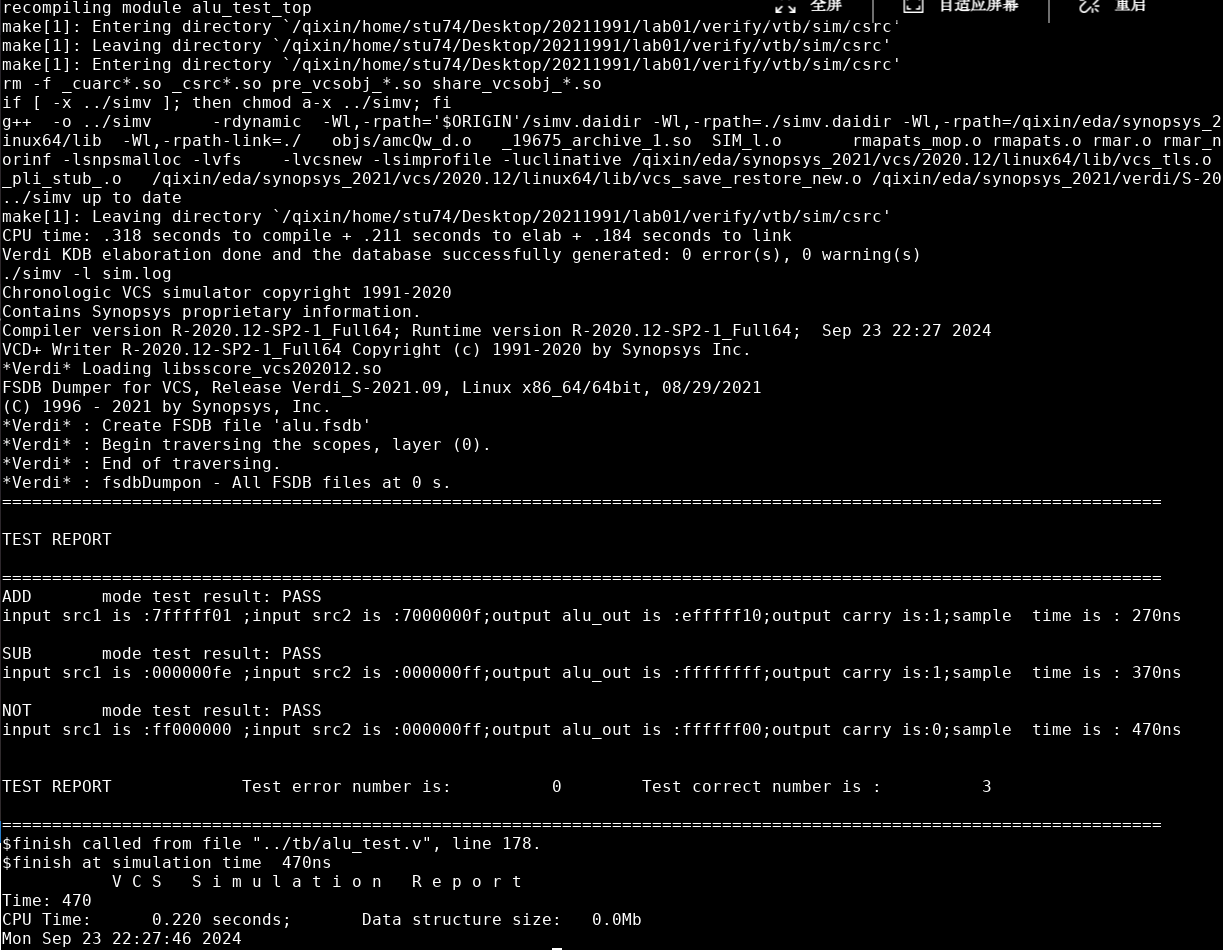
\includegraphics[width=0.8\textwidth]{images/lab01-01.png}
  \caption{lab01 图1}
\end{figure}

\begin{figure}[H]
    \centering
    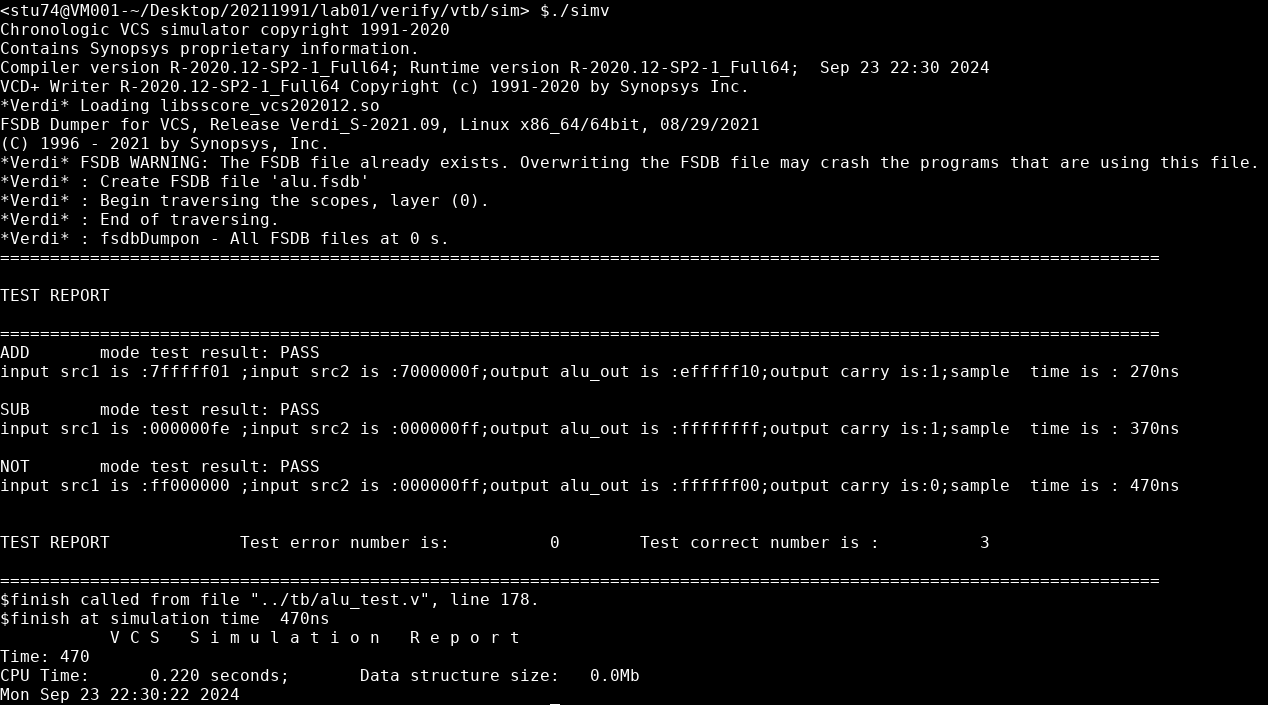
\includegraphics[width=0.8\textwidth]{images/lab01-02.png}
    \caption{lab01 图2}
  \end{figure}

\begin{figure}[H]
    \centering
    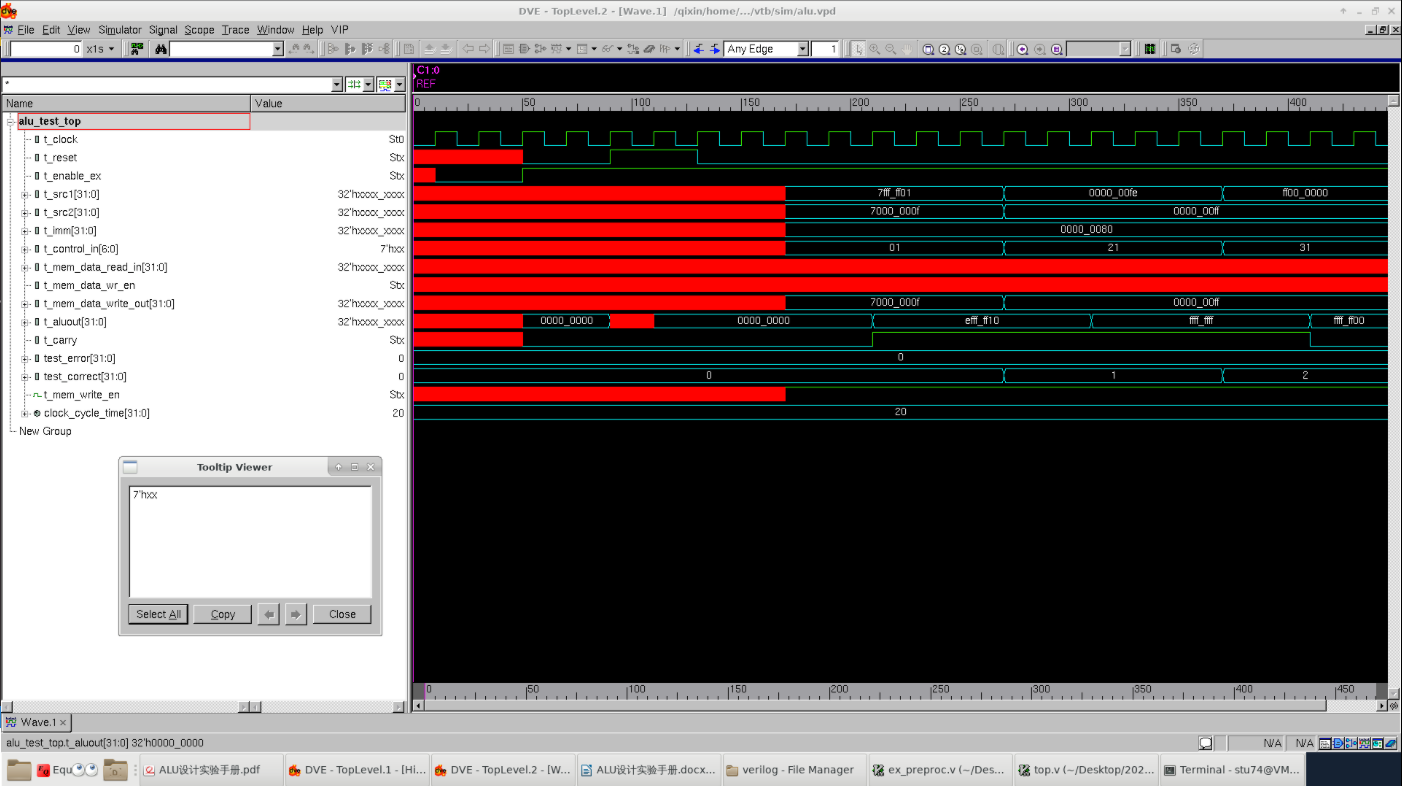
\includegraphics[width=0.8\textwidth]{images/lab01-03.png}
    \caption{lab01 图3}
\end{figure}

\subsection{lab02}

实验目的

通过本次实验,你将:

1. 知道如何编写一个ALU的测试程序。
2. 了解测试程序需要包含哪些组件。

实验步骤

1.	 任务包含共8个部分

Task1  在测试代码中实例化DUT
Task2  产生时钟信号
Task3  使能ALU
Task4  复位ALU
Task5  测试ADD功能并判断是否符合预期,并打印结果
Task6  测试SUB功能并判断是否符合预期,并打印结果 
Task7  测试SHLEFTLOG功能并判断是否符合预期,并打印结果
Task8  生成VPD波形文件

2. Task1在测试代码中实例化DUT

该任务是在测试程序的顶层中,实例化一个ALU模块,并将测试信号连接到ALU模块上。

3. Task2  产生时钟信号

5. Task3  使能ALU

6. Task4  复位ALU

7. Task5  测试ADD功能并判断是否符合预期,并打印结果

编译代码,确认没有错误。

在 \texttt{/sim} 文件夹下使用命令 \texttt{make compile} 编译;使用 \texttt{make simulate} 命令进行仿真,查看终端窗口的打印信息是否与预期一致。 仿真后 ADD 功能应该 PASS。

\begin{figure}[H]
    \centering
    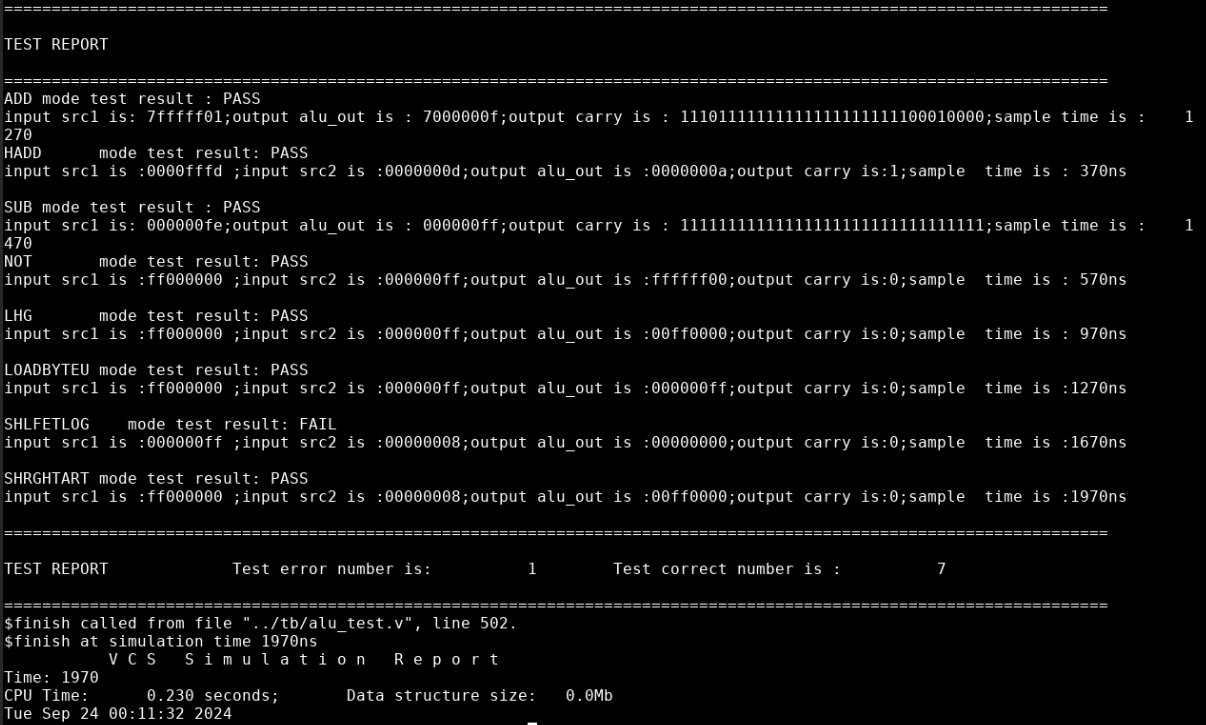
\includegraphics[width=0.8\textwidth]{images/lab02-01.png}
    \caption{lab02 图1}
\end{figure}

8. Task6  测试SUB功能并判断是否符合预期,并打印结果

9. Task7  测试SHLEFTLOG功能并判断是否符合预期,并打印结果

10. Task8  生成VPD波形文件

\begin{figure}[H]
    \centering
    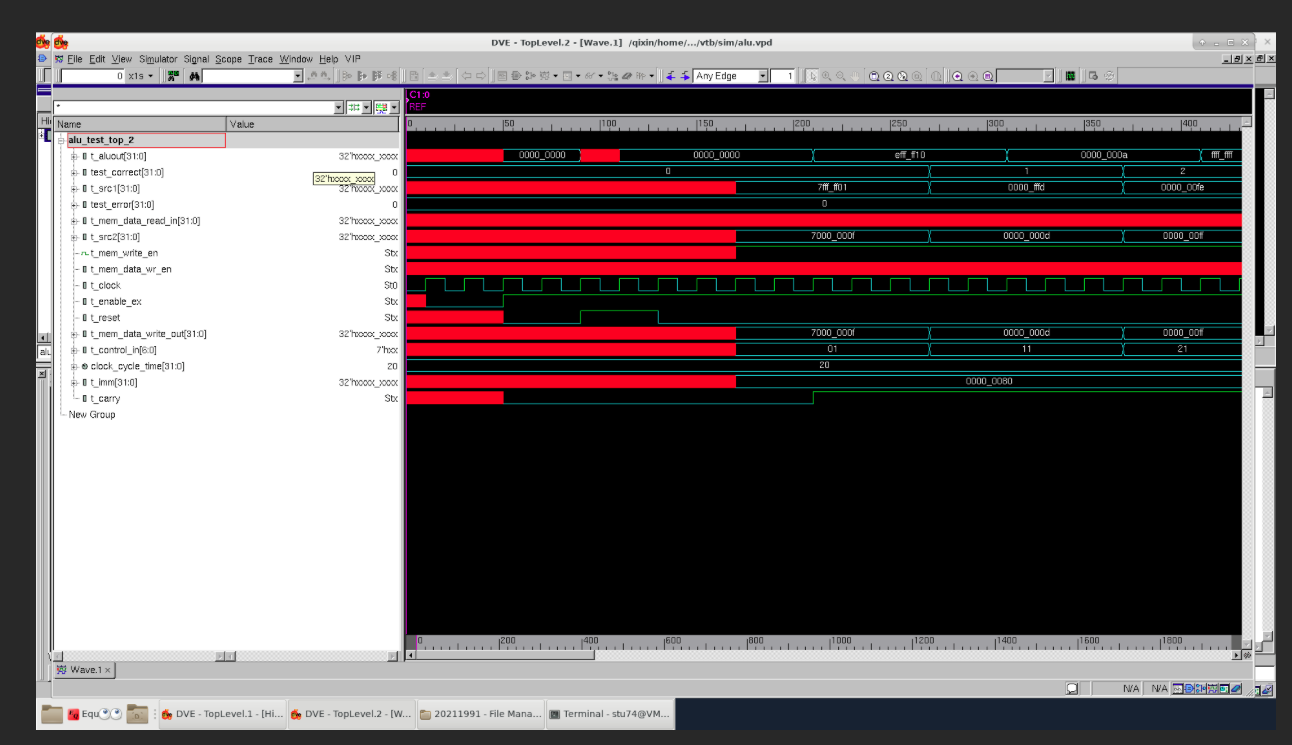
\includegraphics[width=0.8\textwidth]{images/lab02-02.png}
    \caption{lab02 图2}
\end{figure}

随后,点击查看信号全局

\begin{figure}[H]
    \centering
    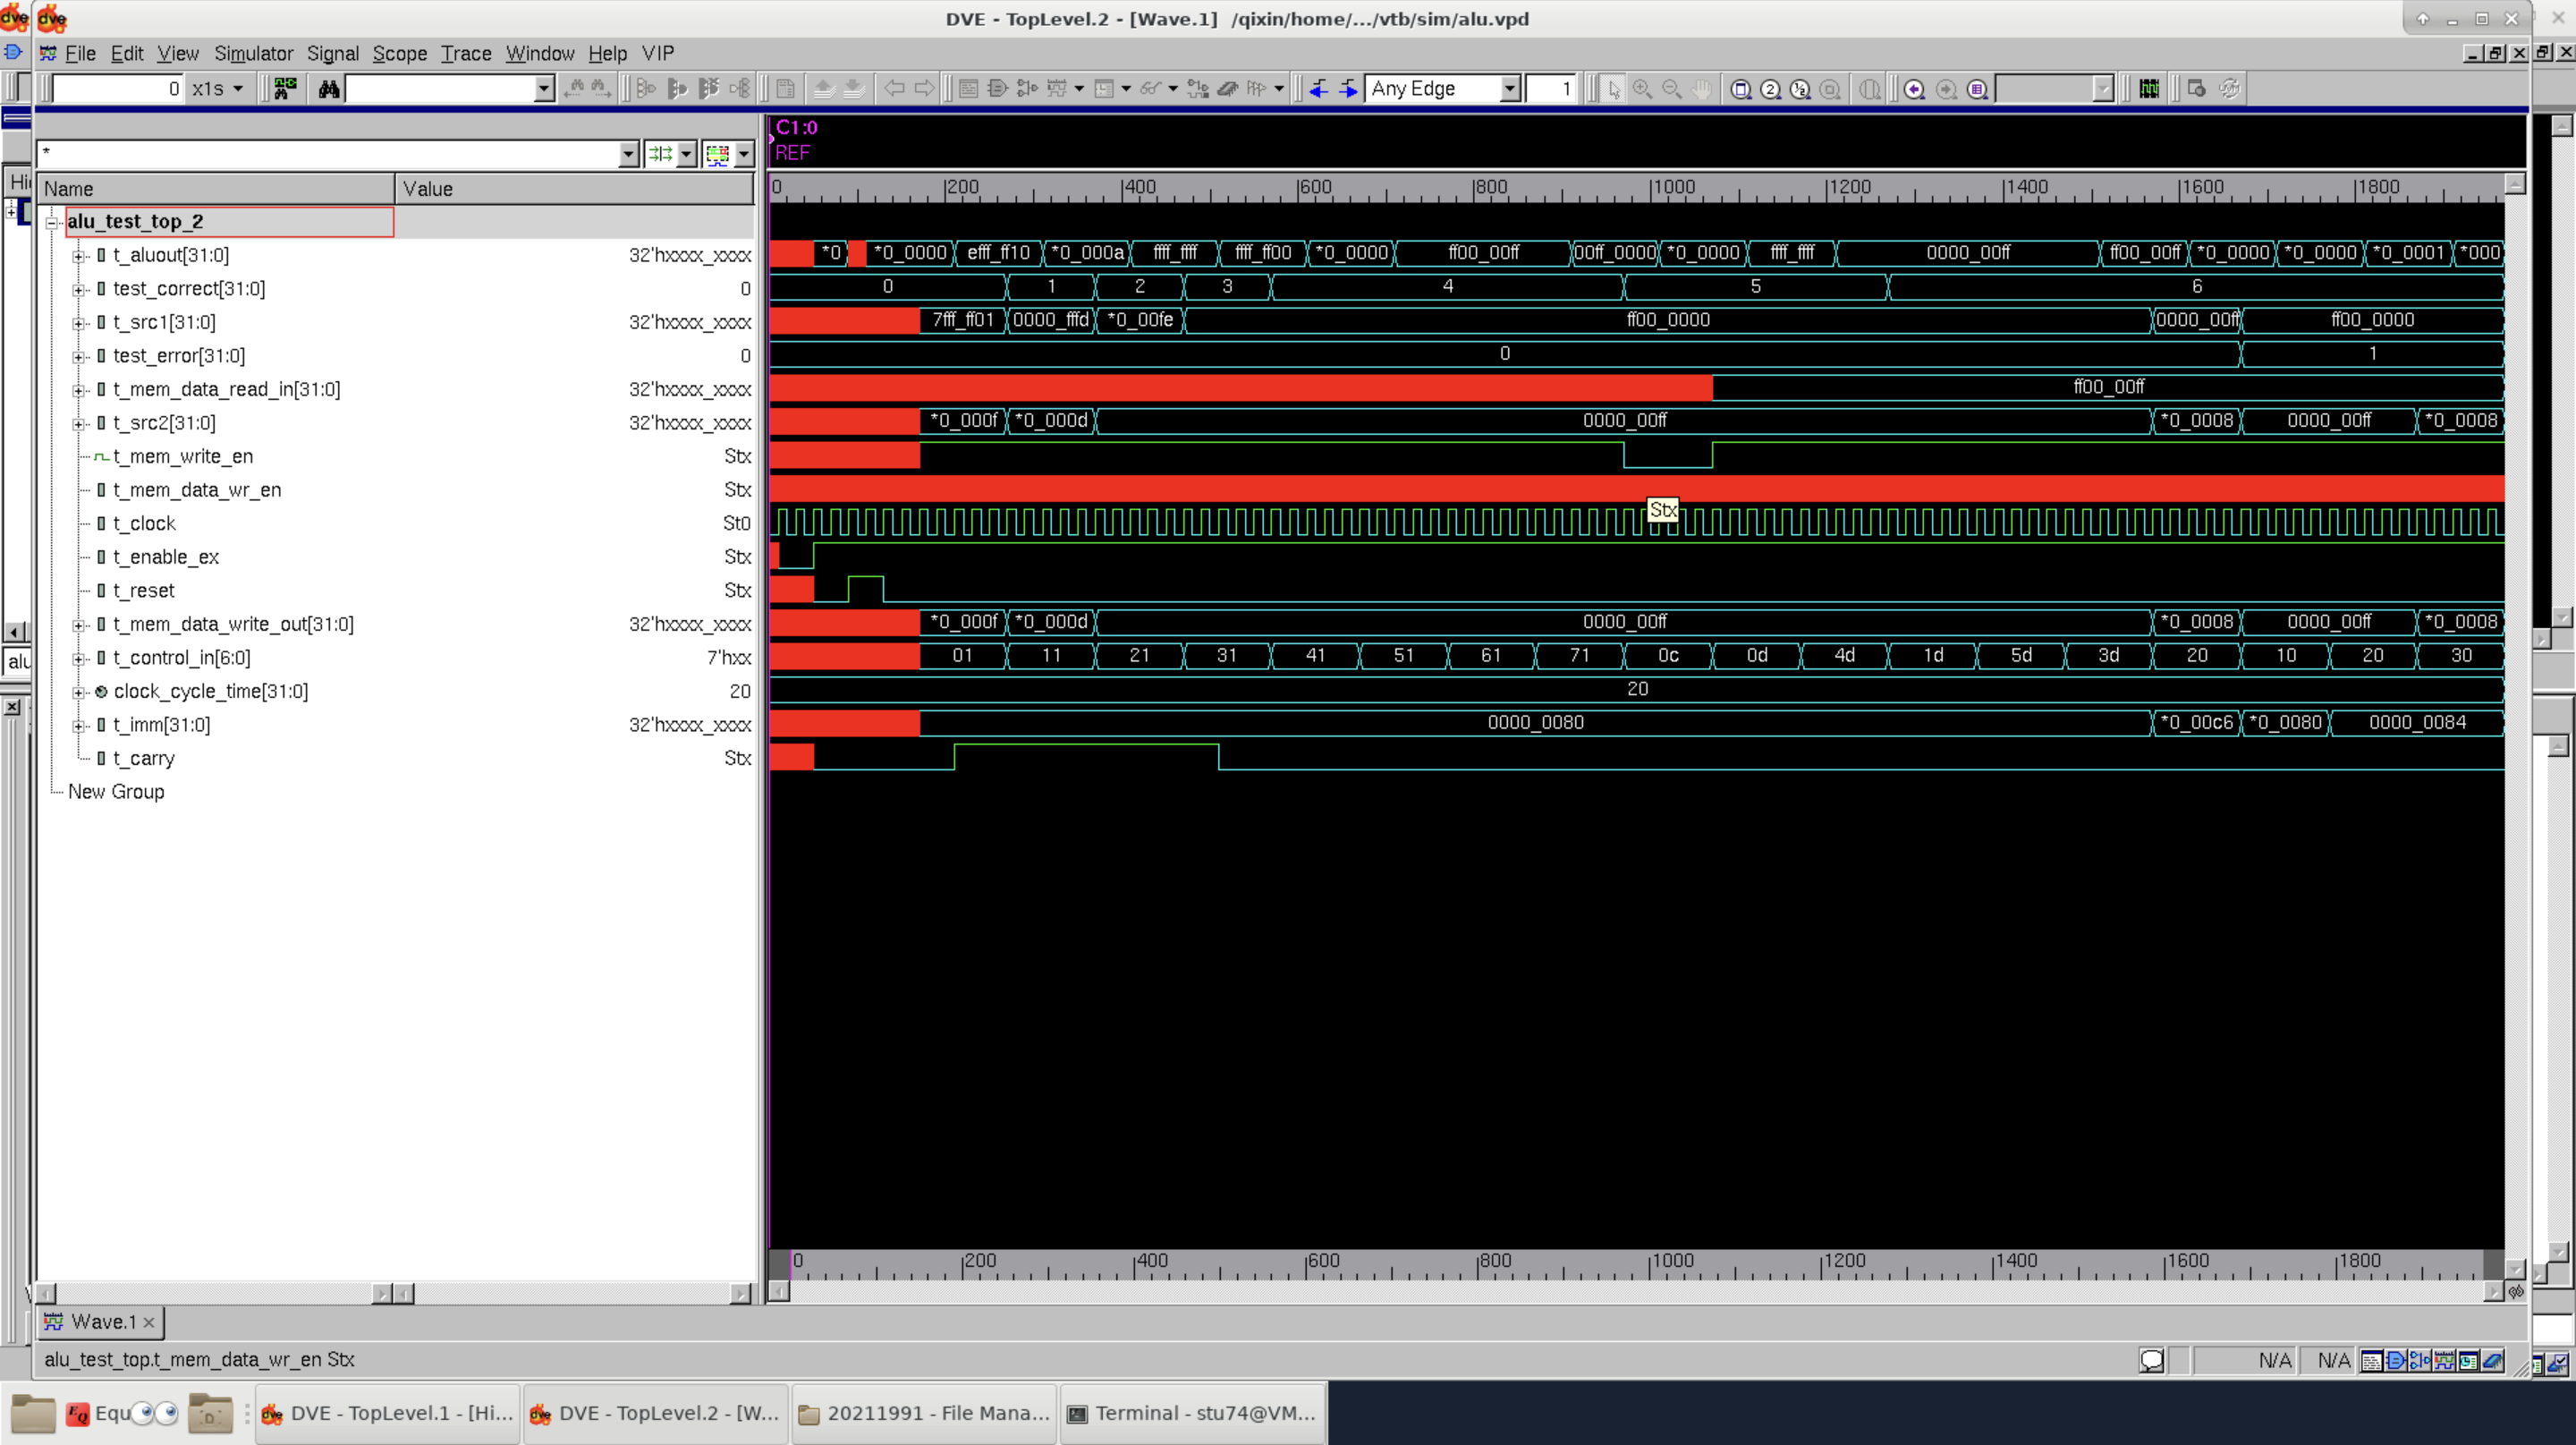
\includegraphics[width=0.8\textwidth]{images/lab02-03.png}
    \caption{lab02 图3}
\end{figure}

\subsection{lab03}

实验目的

1、熟悉使用DC工具的使用方法。
2、熟悉使用TCL脚本使用 DC 工具进行编译和综合。

实验步骤:

1、	进入到dc路径下,启动dc,键入: \texttt{dc\_shell}

2、	在dc\_shell命令框下输入命令: \texttt{source run\_dc.tcl}
注:run\_dc.tcl 是一个tcl脚本,主要实现了Design Compiler的详细步骤。

3、	在命令栏输入 \texttt{report\_timing}

% 需要注意的是,由于暂时未知的某种原因,实际运行的结果与实验指导书的结果有所不同。

结果如下(结果为正,时序正常):

% \begin{figure}[H]
%     \centering
%     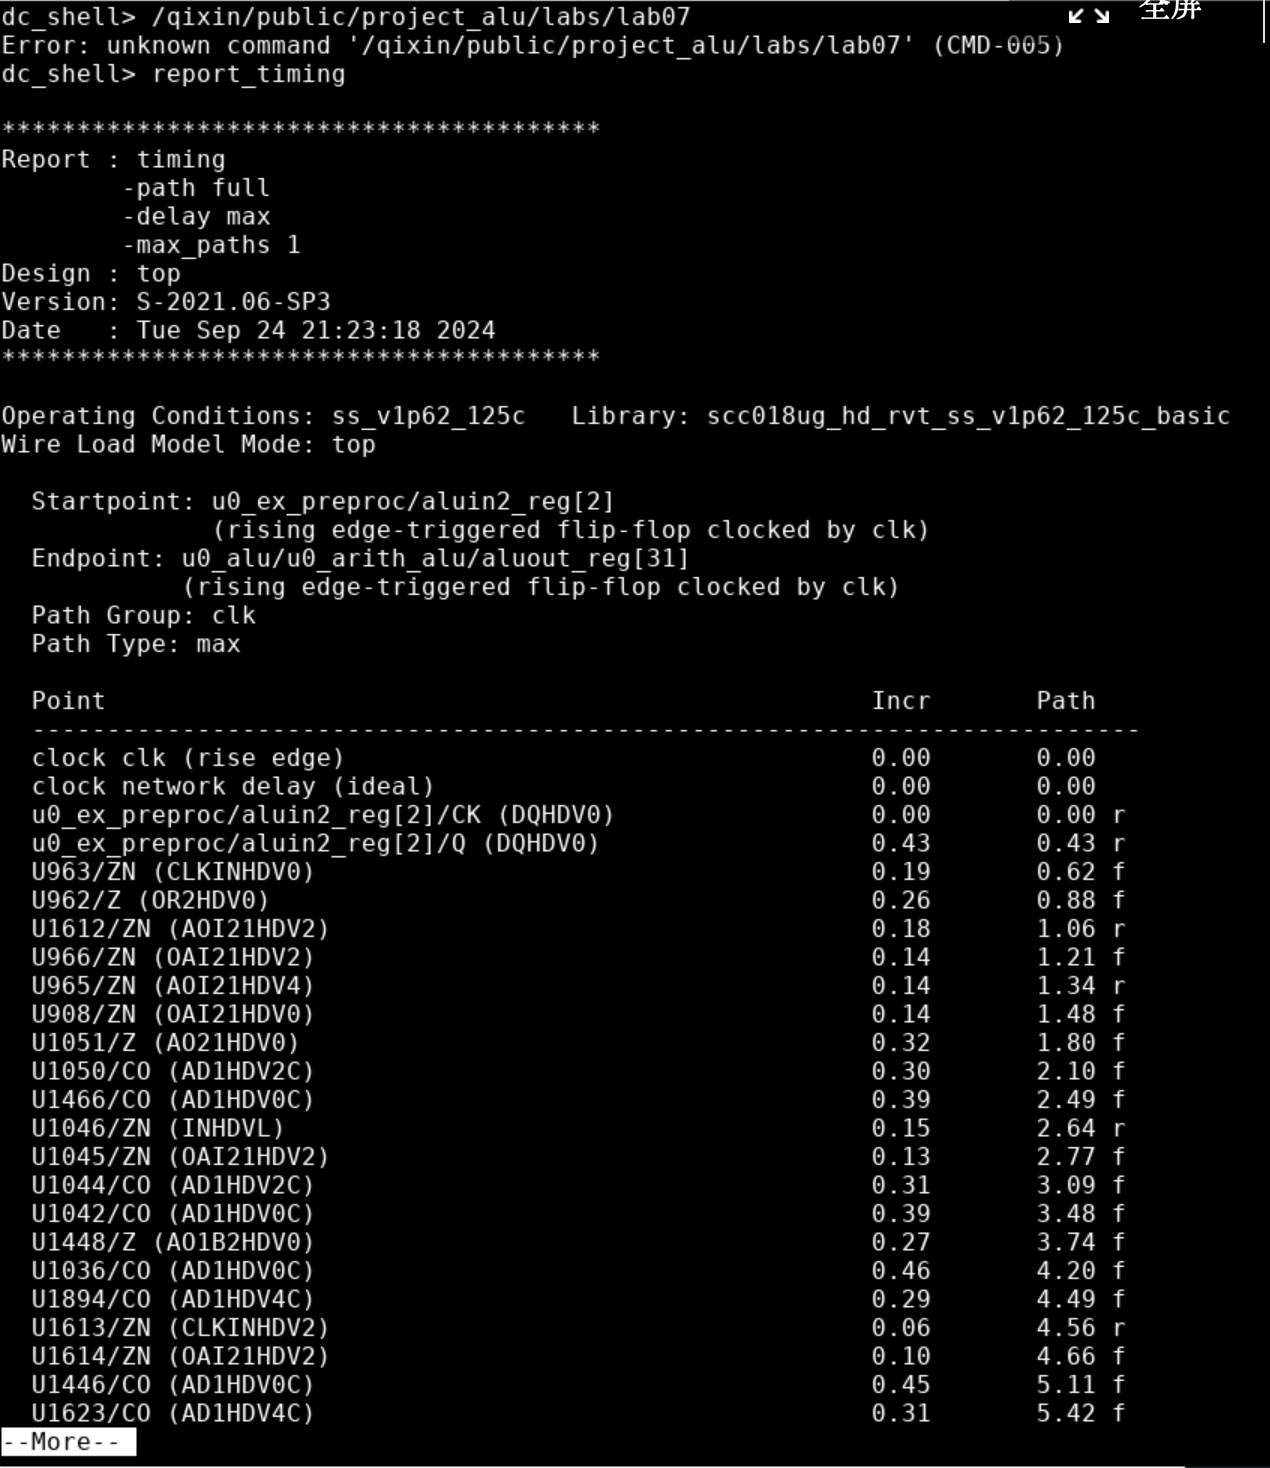
\includegraphics[width=0.8\textwidth]{images/lab03-01.png}
%     \caption{lab03 图1}
% \end{figure}

% \begin{figure}[H]
%     \centering
%     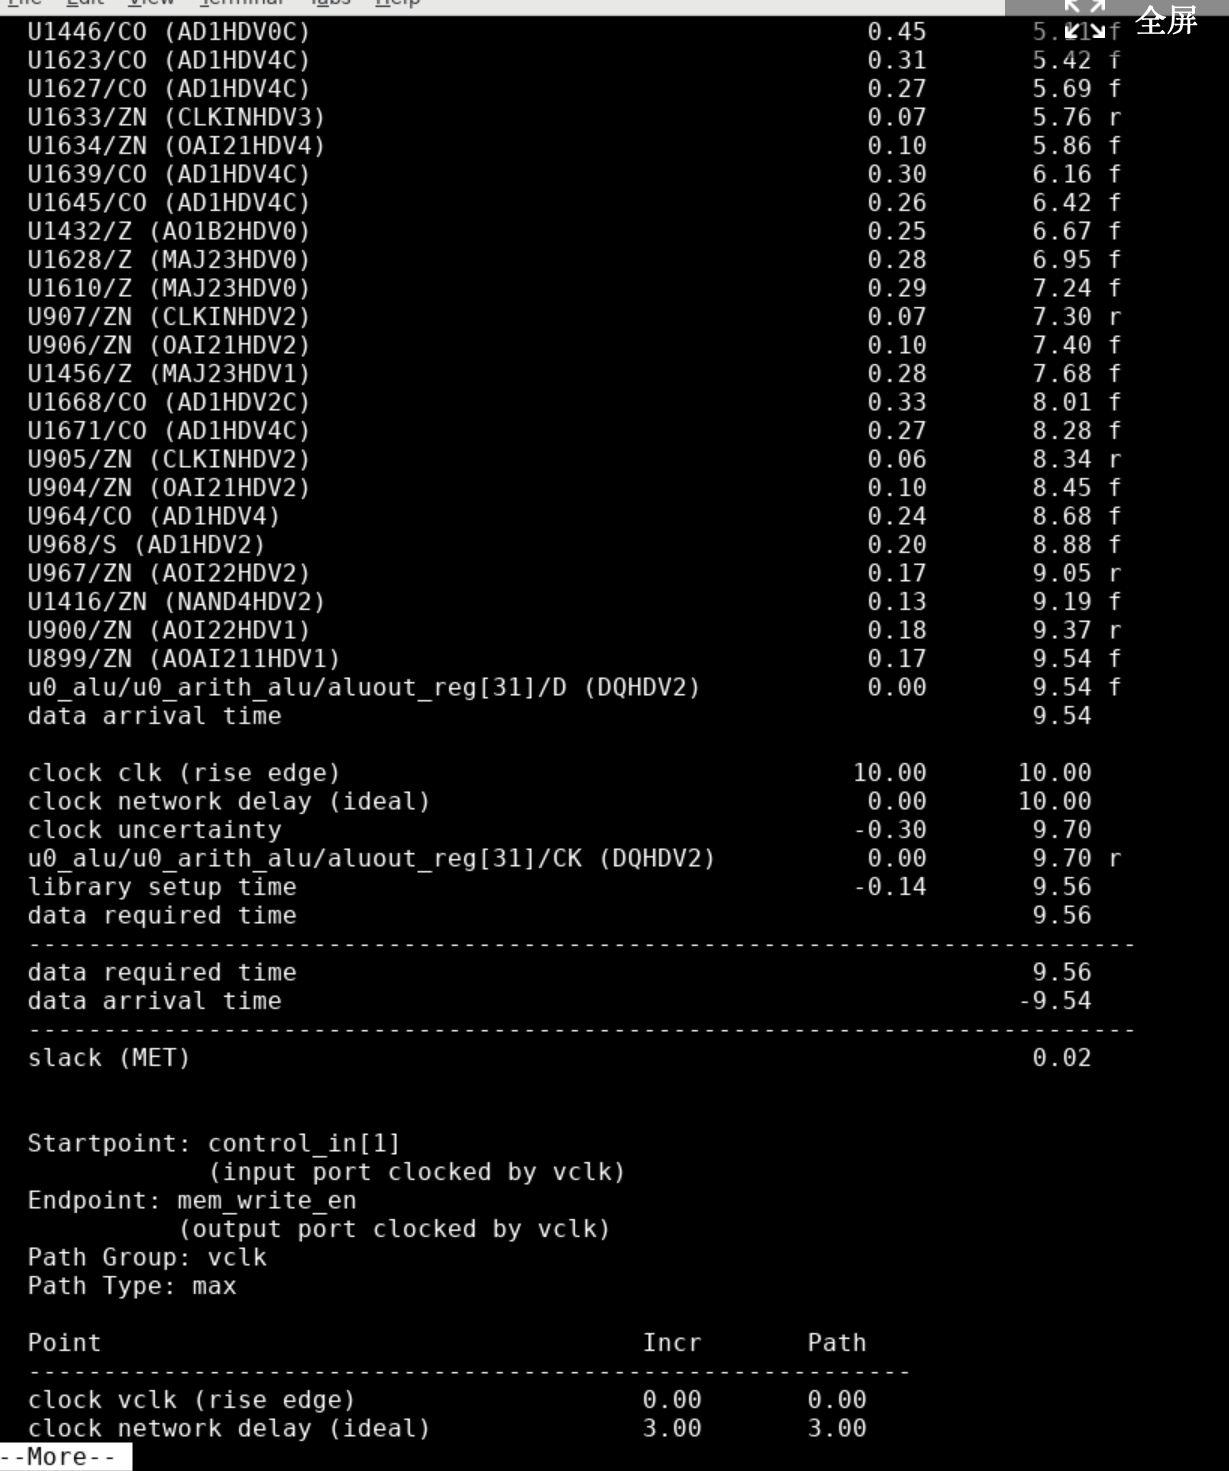
\includegraphics[width=0.8\textwidth]{images/lab03-02.png}
%     \caption{lab03 图2}
% \end{figure}

\begin{figure}[H]
    \centering
    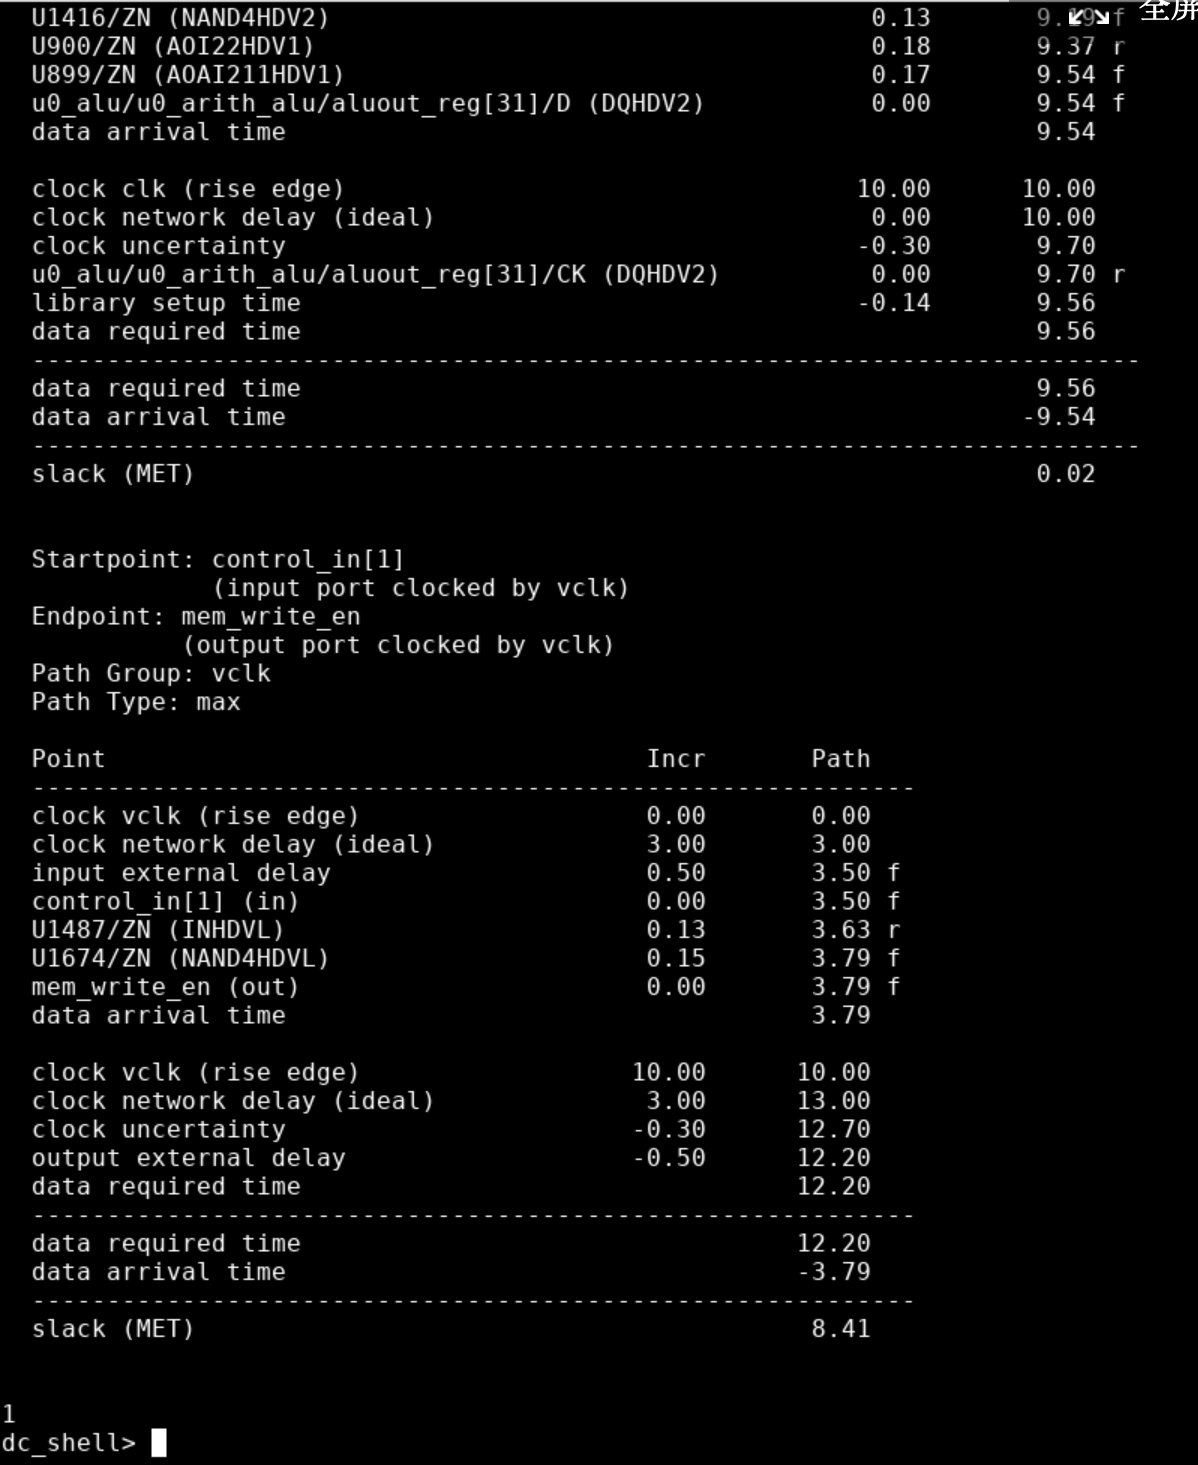
\includegraphics[width=0.8\textwidth]{images/lab03-03.png}
    \caption{lab03 图3}
\end{figure}

\subsubsection{Lab03 Q\&A}

\texttt{run\_da.tcl} 中三个 DC 综合命令的意义:

1. \texttt{compile\_ultra}:综合,使用目标库中的最高级别的综合选项。
2. \texttt{compile\_ultra -incremental}:综合,使用目标库中的最高级别的综合选项,并增量综合。
3. \texttt{optimize\_netlist -area}:优化综合后的电路,以面积为目标。

\texttt{alu.sdc} 文件中每条命令是什么意思

解释:

1. \texttt{create\_clock -name clk -period 10 -waveform \{0 5\} [get\_ports clock]}:创建时钟,时钟名为 \texttt{clk},周期为10ns,波形为 \texttt{0 5},时钟源为 \texttt{clock} 端口。
2. \texttt{create\_clock -name vclk -period 10 -waveform \{0 5\}}:创建时钟,时钟名为 \texttt{vclk},周期为10ns,波形为 \texttt{0 5}。
3. \texttt{set\_clock\_uncertainty -setup 0.3 [all\_clocks]}:设置时钟不确定性,setup为0.3ns。
4. \texttt{set\_clock\_uncertainty -hold 0.2 [all\_clocks]}:设置时钟不确定性,hold为0.2ns。
5. \texttt{set\_input\_delay  -add\_delay 0.5 -clock vclk [all\_inputs]}:设置输入延迟,增加延迟0.5ns,时钟为 \texttt{vclk},所有输入。
6. \texttt{set\_output\_delay -add\_delay 0.5 -clock vclk [all\_outputs]}:设置输出延迟,增加延迟0.5ns,时钟为 \texttt{vclk},所有输出。
7. \texttt{set\_input\_delay  -add\_delay 0.5 -clock clk [all\_inputs]}:设置输入延迟,增加延迟0.5ns,时钟为 \texttt{clk},所有输入。
8. \texttt{set\_output\_delay -add\_delay 0.5 -clock clk [all\_outputs]}:设置输出延迟,增加延迟0.5ns,时钟为 \texttt{clk},所有输出。
9. \texttt{set\_clock\_latency 3 [get\_clocks vclk]}:设置时钟延迟,时钟为 \texttt{vclk},延迟为3ns。

\texttt{slack} 指标代表什么意思

解释:

在时序分析中,slack 是一个关键指标,用来衡量设计中时序路径的时序裕量。它表示信号在特定路径上是否按时到达或者是否存在时序违反。如果 slack 值为正数,则表明设计满足时序要求;如果 slack 值为负数,则表示存在时序违例。

1. \texttt{slack (MET) 0.02}:slack指标为0.02ns,MET表示满足时序要求。
2. \texttt{slack (MET) 8.41}:slack指标为8.41ns,MET表示满足时序要求。

\subsection{lab04}

实验目的

1、验证综合前后的网表逻辑等价性检查。
2、验证综合后的网表与绕线后的网表逻辑等价性检查。

实验步骤

Lab1 rtl代码与DC综合之后的网表:

1、	cd进入到fm目录下进行形式验证

2、	在fm目录下有 \texttt{run\_R2G.tcl} 脚本,

3、	运行\texttt{fm\_shell, source run\_R2G.tcl} 脚本进行形式验证

4、	运行脚本后,查看结果:

\begin{figure}[H]
    \centering
    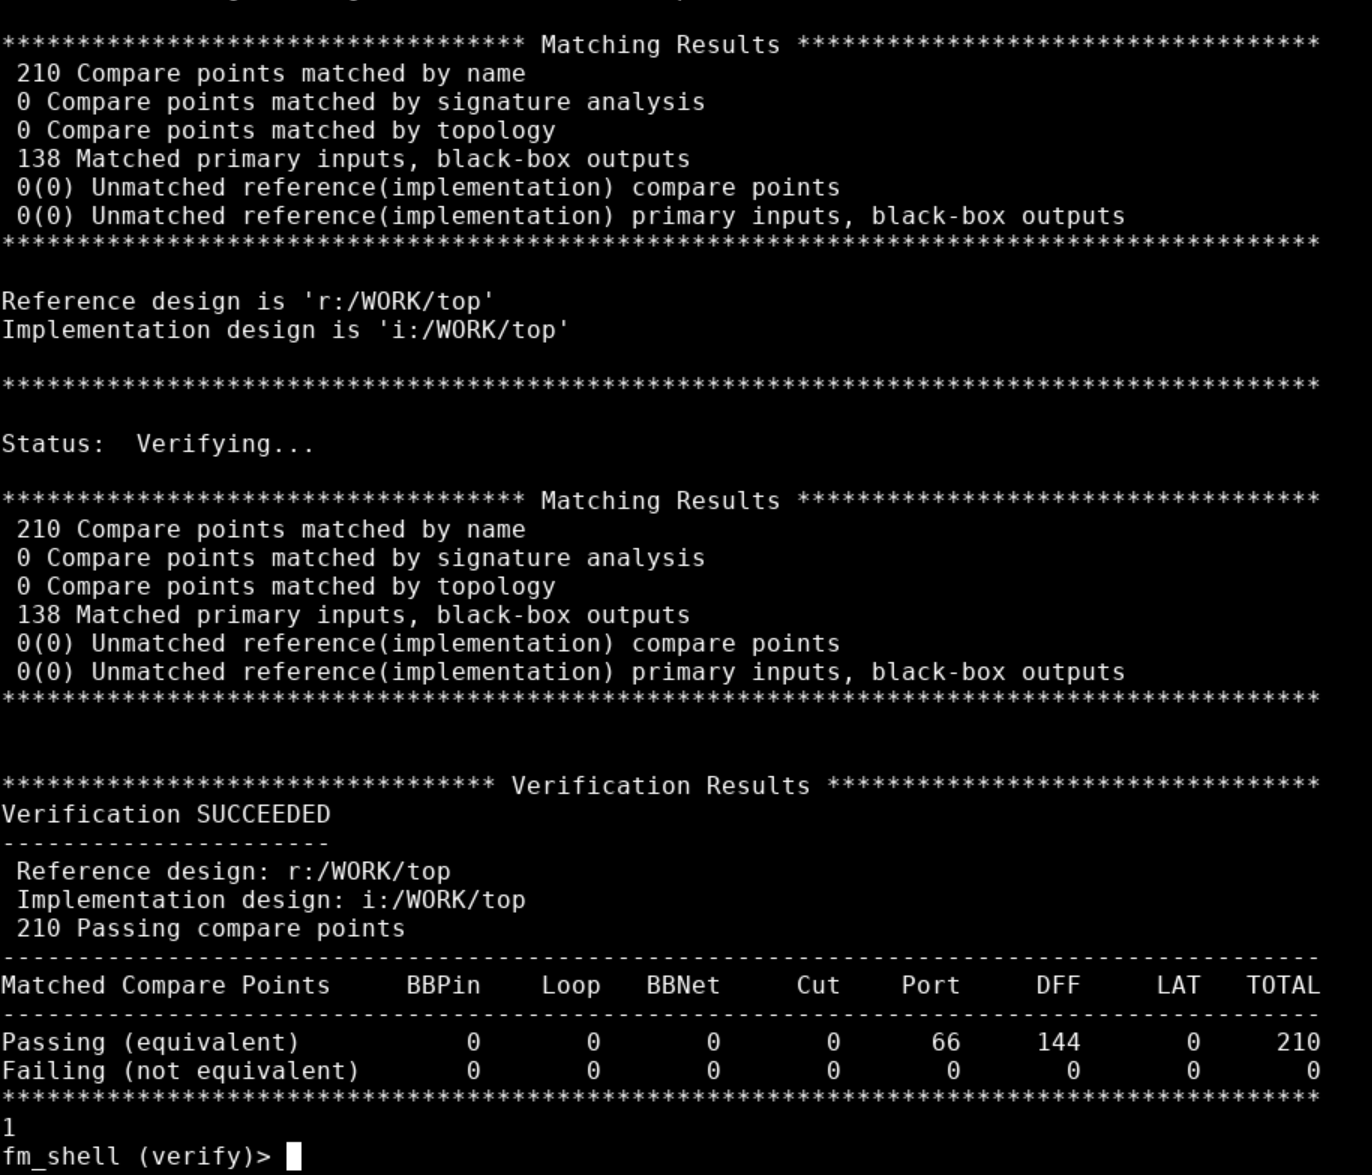
\includegraphics[width=0.8\textwidth]{images/lab04-01.png}
    \caption{lab04 图1}
\end{figure}

Lab2 DC综合之后的网表和route之后的网表:

1、	在fm目录下有 \texttt{run\_G2G.tcl} 脚本

2、	在fm目录下有 \texttt{run\_G2G.tcl} 脚本,

3、	运行\texttt{fm\_shell, source run\_G2G.tcl} 脚本进行形式验证

4、	运行脚本后,查看结果:

\begin{figure}[H]
    \centering
    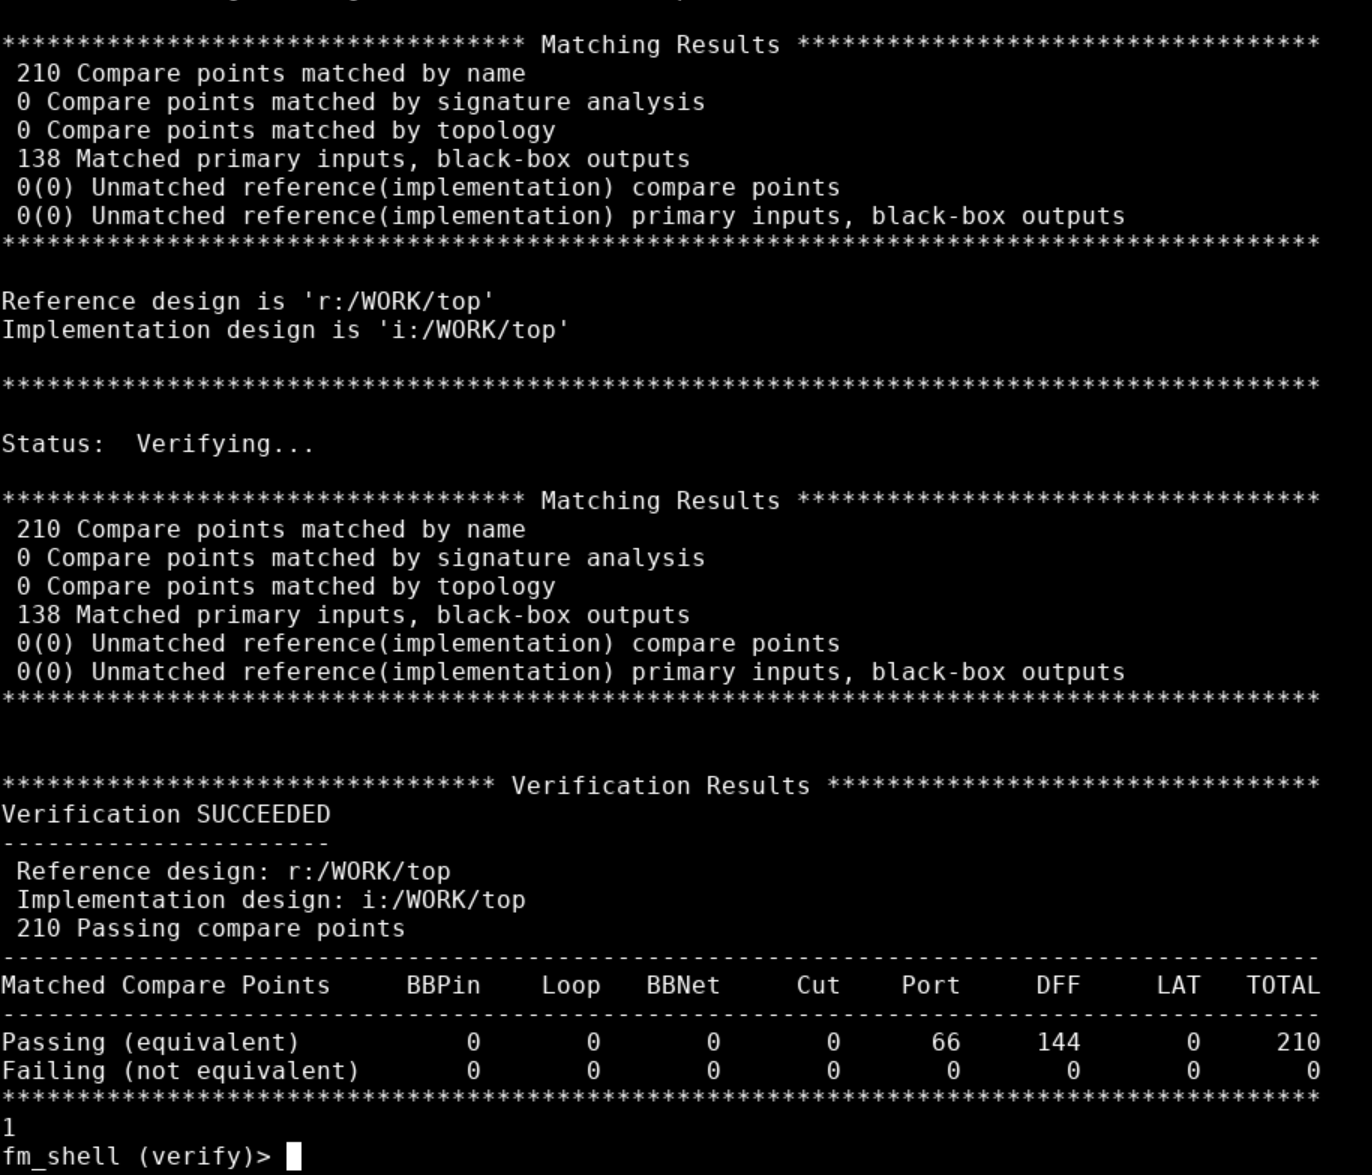
\includegraphics[width=0.8\textwidth]{images/lab04-01.png}
    \caption{lab04 图1}
\end{figure}

\subsubsection{lab04 Q\&A}

什么是形式验证?

解释:

形式验证(Formal Verification)是一种用于验证硬件设计或软件系统是否符合其规格说明的技术,它基于数学证明的方式,确保设计在所有可能的输入情况下都满足预期的行为。与传统的仿真验证不同,形式验证不依赖测试向量或具体输入,而是对设计进行系统性和彻底的检查。

\texttt{run\_G2G.tcl} 与 \texttt{run\_R2G.tcl} 这两文件有何不同,目的是什么?

解释:

\texttt{run\_G2G.tcl} 脚本主要用于门级网表验证(Gate-to-Gate,简称 G2G),即在综合后对门级网表与布线信息进行验证。该脚本读取门级网表和布线文件,并通过匹配和验证来确保综合后的门级设计与布线设计一致。
\texttt{run\_R2G.tcl} 脚本用于 RTL-to-Gate(R2G)验证,即在综合前后的 RTL 代码与门级网表之间进行验证,确保 RTL 代码与综合后的门级网表行为一致。这是设计验证流程中的关键步骤,保证综合前后的功能没有发生变化。

\subsection{lab05}

实验目的

1、掌握QRC寄生参数提取。

2、掌握数字后端tempus的使用。

实验步骤

Lab1 QRC参数提取:

1、	在rc目录下创建 \texttt{qrc\_tech\_dir} 目录,准备 \texttt{corner.defs} 文件,内容如下
 
2、	在qrc目录下创建一个techlib.defs文件,用来定义RC techfile路径:
 
3、	在qrc目录下创建一个qrc.cmd文件, 内容如下

取RC时考虑耦合电容:
 
读取的lef和def文件:
 
指定log文件和输出文件类型:
 
指定layer mapping内容,把innovus里的层和qrcTechFile里的层对应起来:
 
定义所采用的corner和输出路径:
 
4、 输入命令后即可得到抽取的spef文件:
 
进入 \texttt{qrc\_test}目录查看结果:

Lab2 Tempus流程:

1、	抽取qrc参数之后,启动tempus

在sta目录下进行,启动方式:在terminal键入 \texttt{tempus -eco}

2、	导入时序文件

a)读入时序信息
 
b)读入网表
 
c)指定当前design
 
d)读入RC寄生参数信息
 
e)检查Annotated coverage
 
real nets中的complete nets需要保证100\% coverage

\begin{figure}[H]
    \centering
    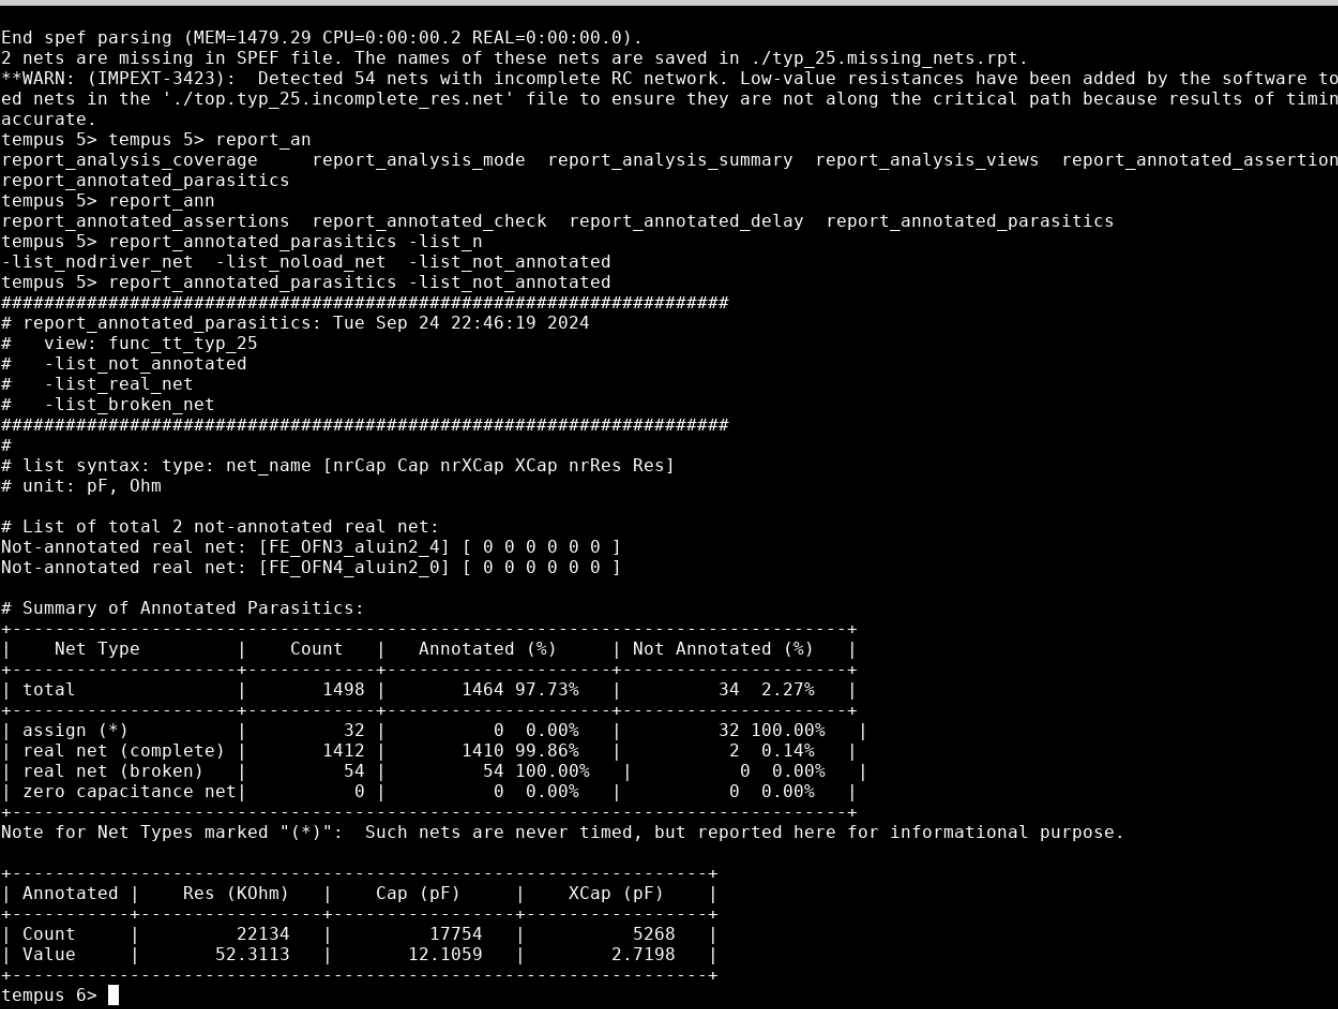
\includegraphics[width=0.8\textwidth]{images/lab05-01.png}
    \caption{lab05 图1}
\end{figure}
 
3、	创建时序路径
 
4、	设置时序分析模式和参数
 
cppr共同路径悲观去除,算delay需要把SI模式打开,设置report报告显示几项重要数据。

5、	产生时序报告

a)产生时序报告前,先运行 \texttt{update\_timing -full}
 
b)产生整体的时序报告,结果存入到\texttt{all\_summary.rpt} 
 
打开报告:

\begin{figure}[H]
    \centering
    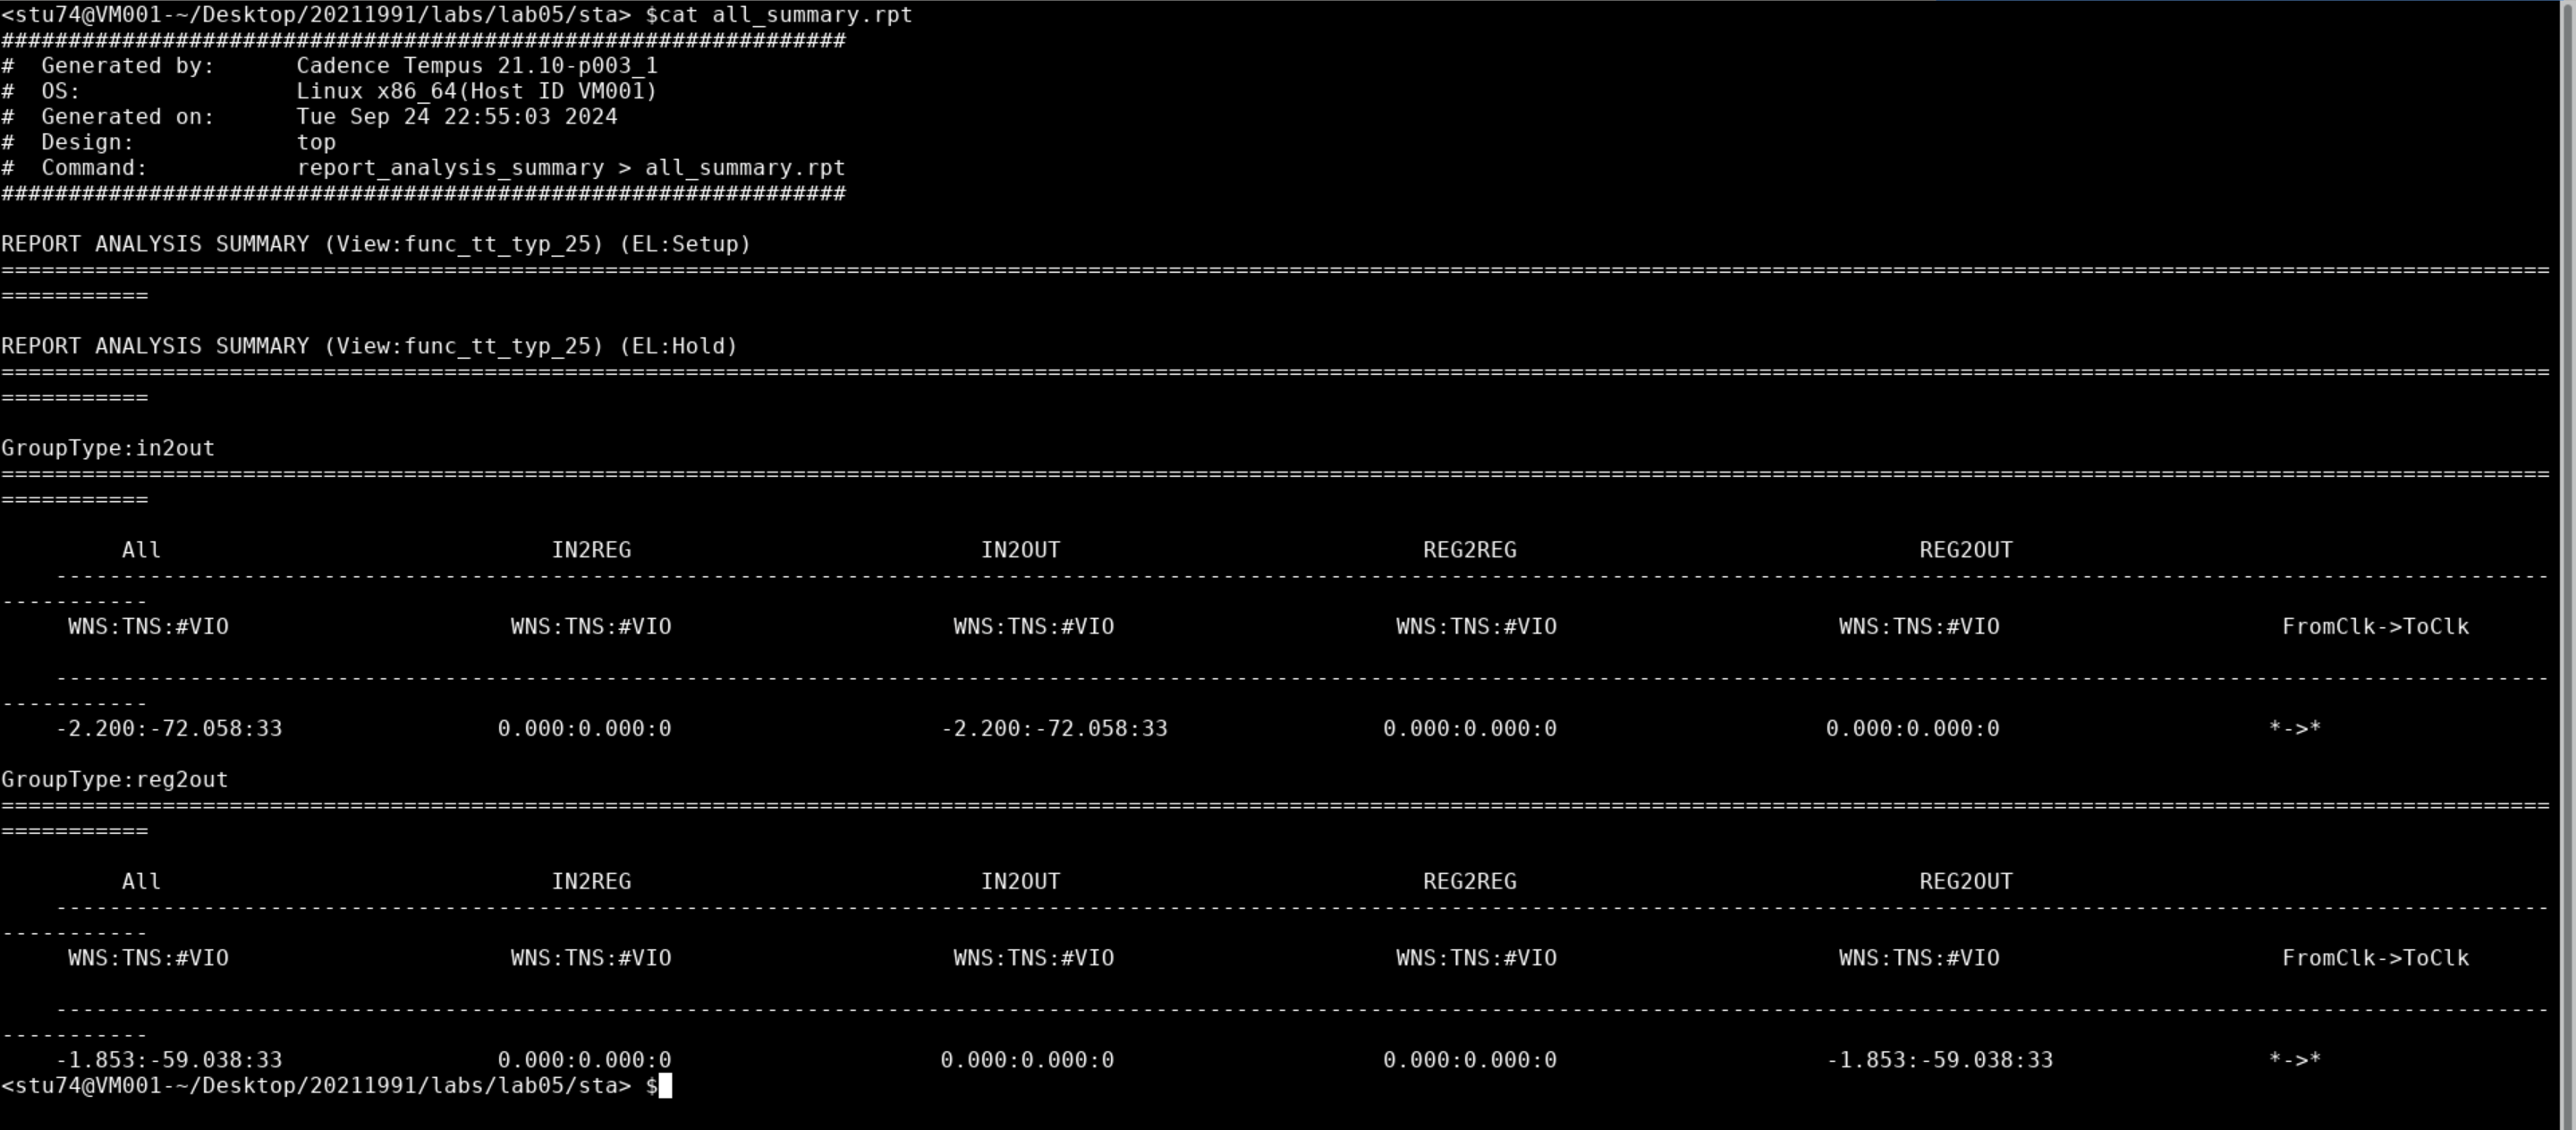
\includegraphics[width=0.8\textwidth]{images/lab05-02.png}
    \caption{lab05 图2}
\end{figure}
 
其中,setup无违例报告,hold有两条违例,但是我们只看reg2reg的违例,故该两条可以忽略。

c)产生setup的时序报告,结果存入到\texttt{late\_gba\_summary.rpt}(late报告的是setup violation,默认GBA分析方式为默认模式)

\begin{figure}[H]
    \centering
    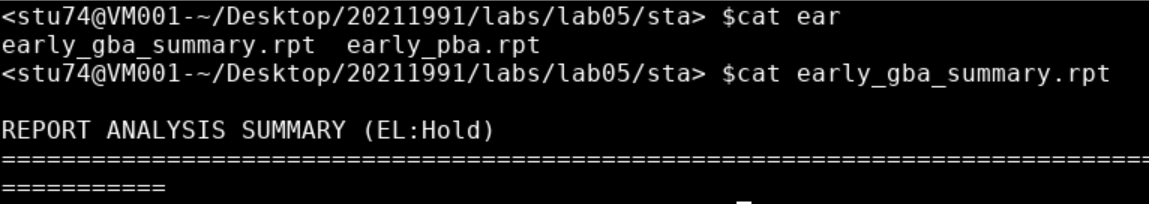
\includegraphics[width=0.8\textwidth]{images/lab05-03.png}
    \caption{lab05 图3}
\end{figure}

(无违例)

d)产生hold的时序报告,结果存入到\texttt{early\_gba\_summary.rpt}(early报告的是hold violation,默认GBA分析方式为默认模式)
 
(无违例)

e)产生PBA模式下的时序报告:
 
\begin{figure}[H]
    \centering
    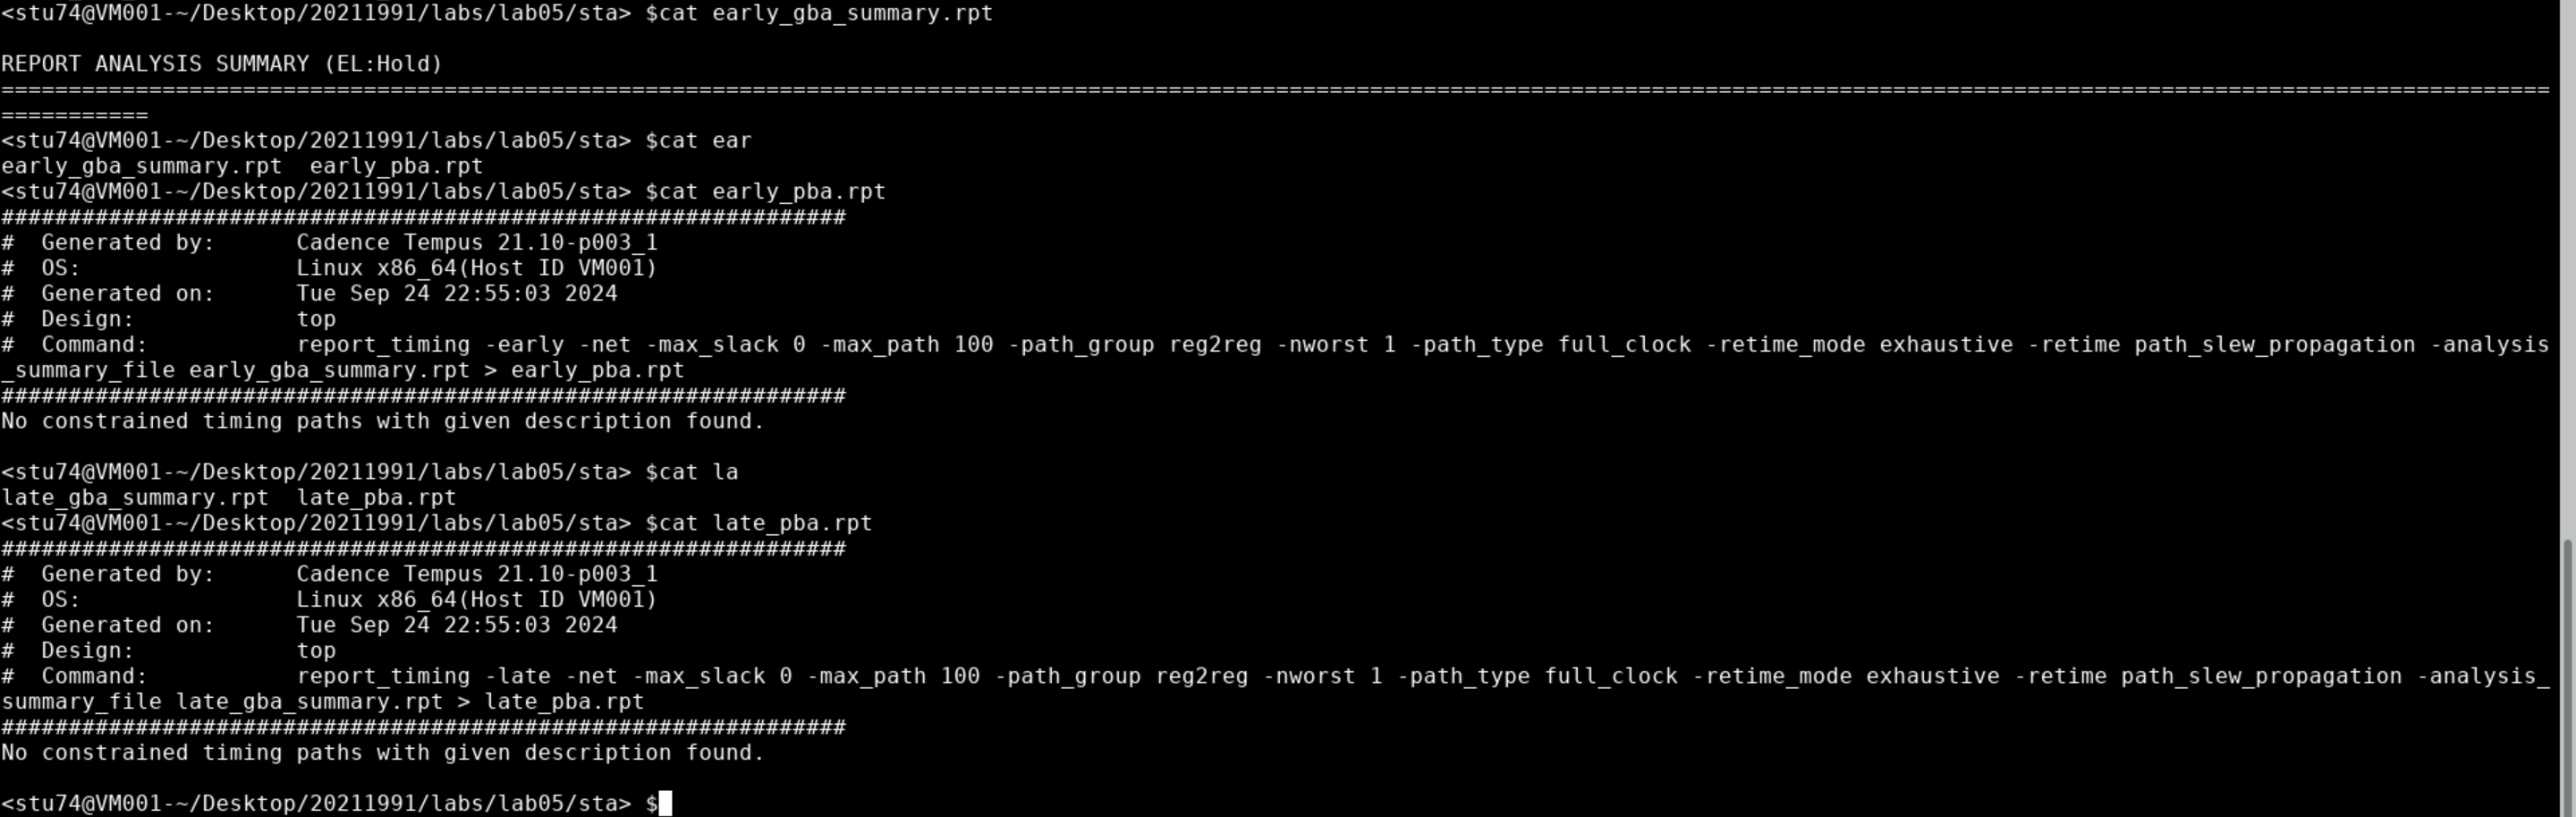
\includegraphics[width=0.8\textwidth]{images/lab05-04.png}
    \caption{lab05 图4}
\end{figure} 
 
(无违例)

f)产生DRV违例报告

\begin{figure}[H]
    \centering
    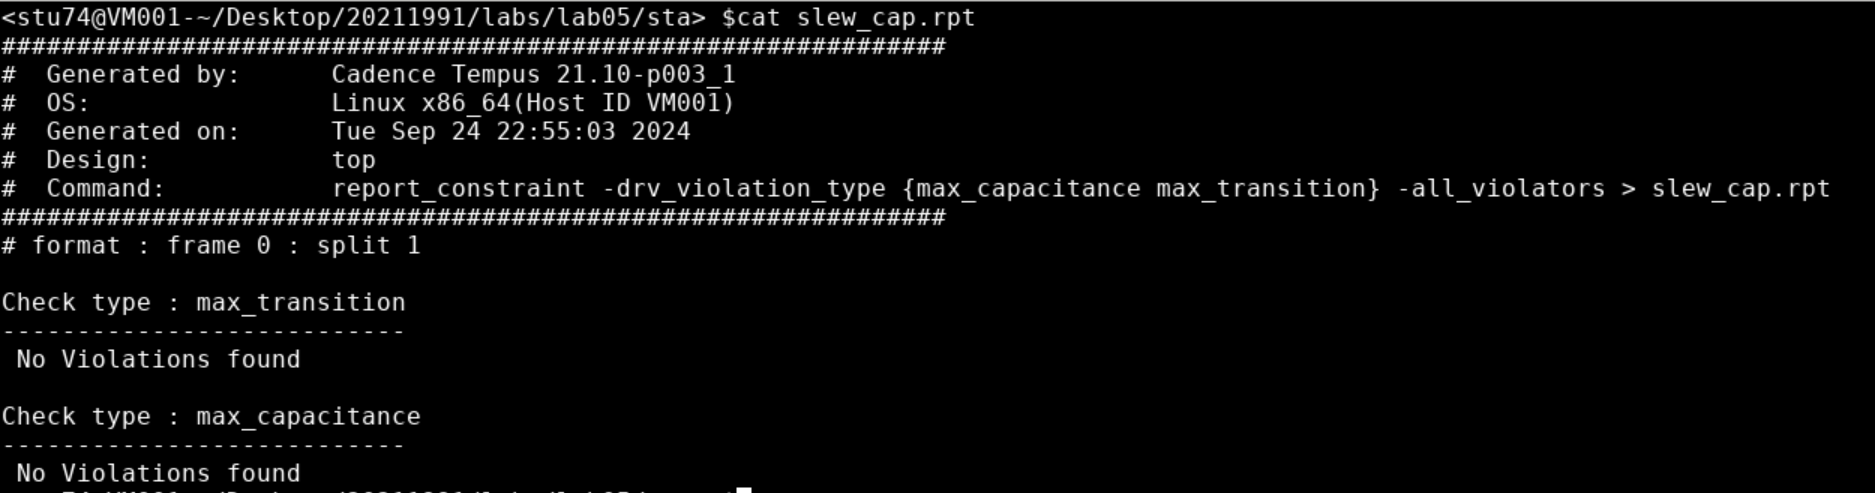
\includegraphics[width=0.8\textwidth]{images/lab05-05.png}
    \caption{lab05 图5}
\end{figure}
 
(无违例)

g)产生noise违例报告

\begin{figure}[H]
    \centering
    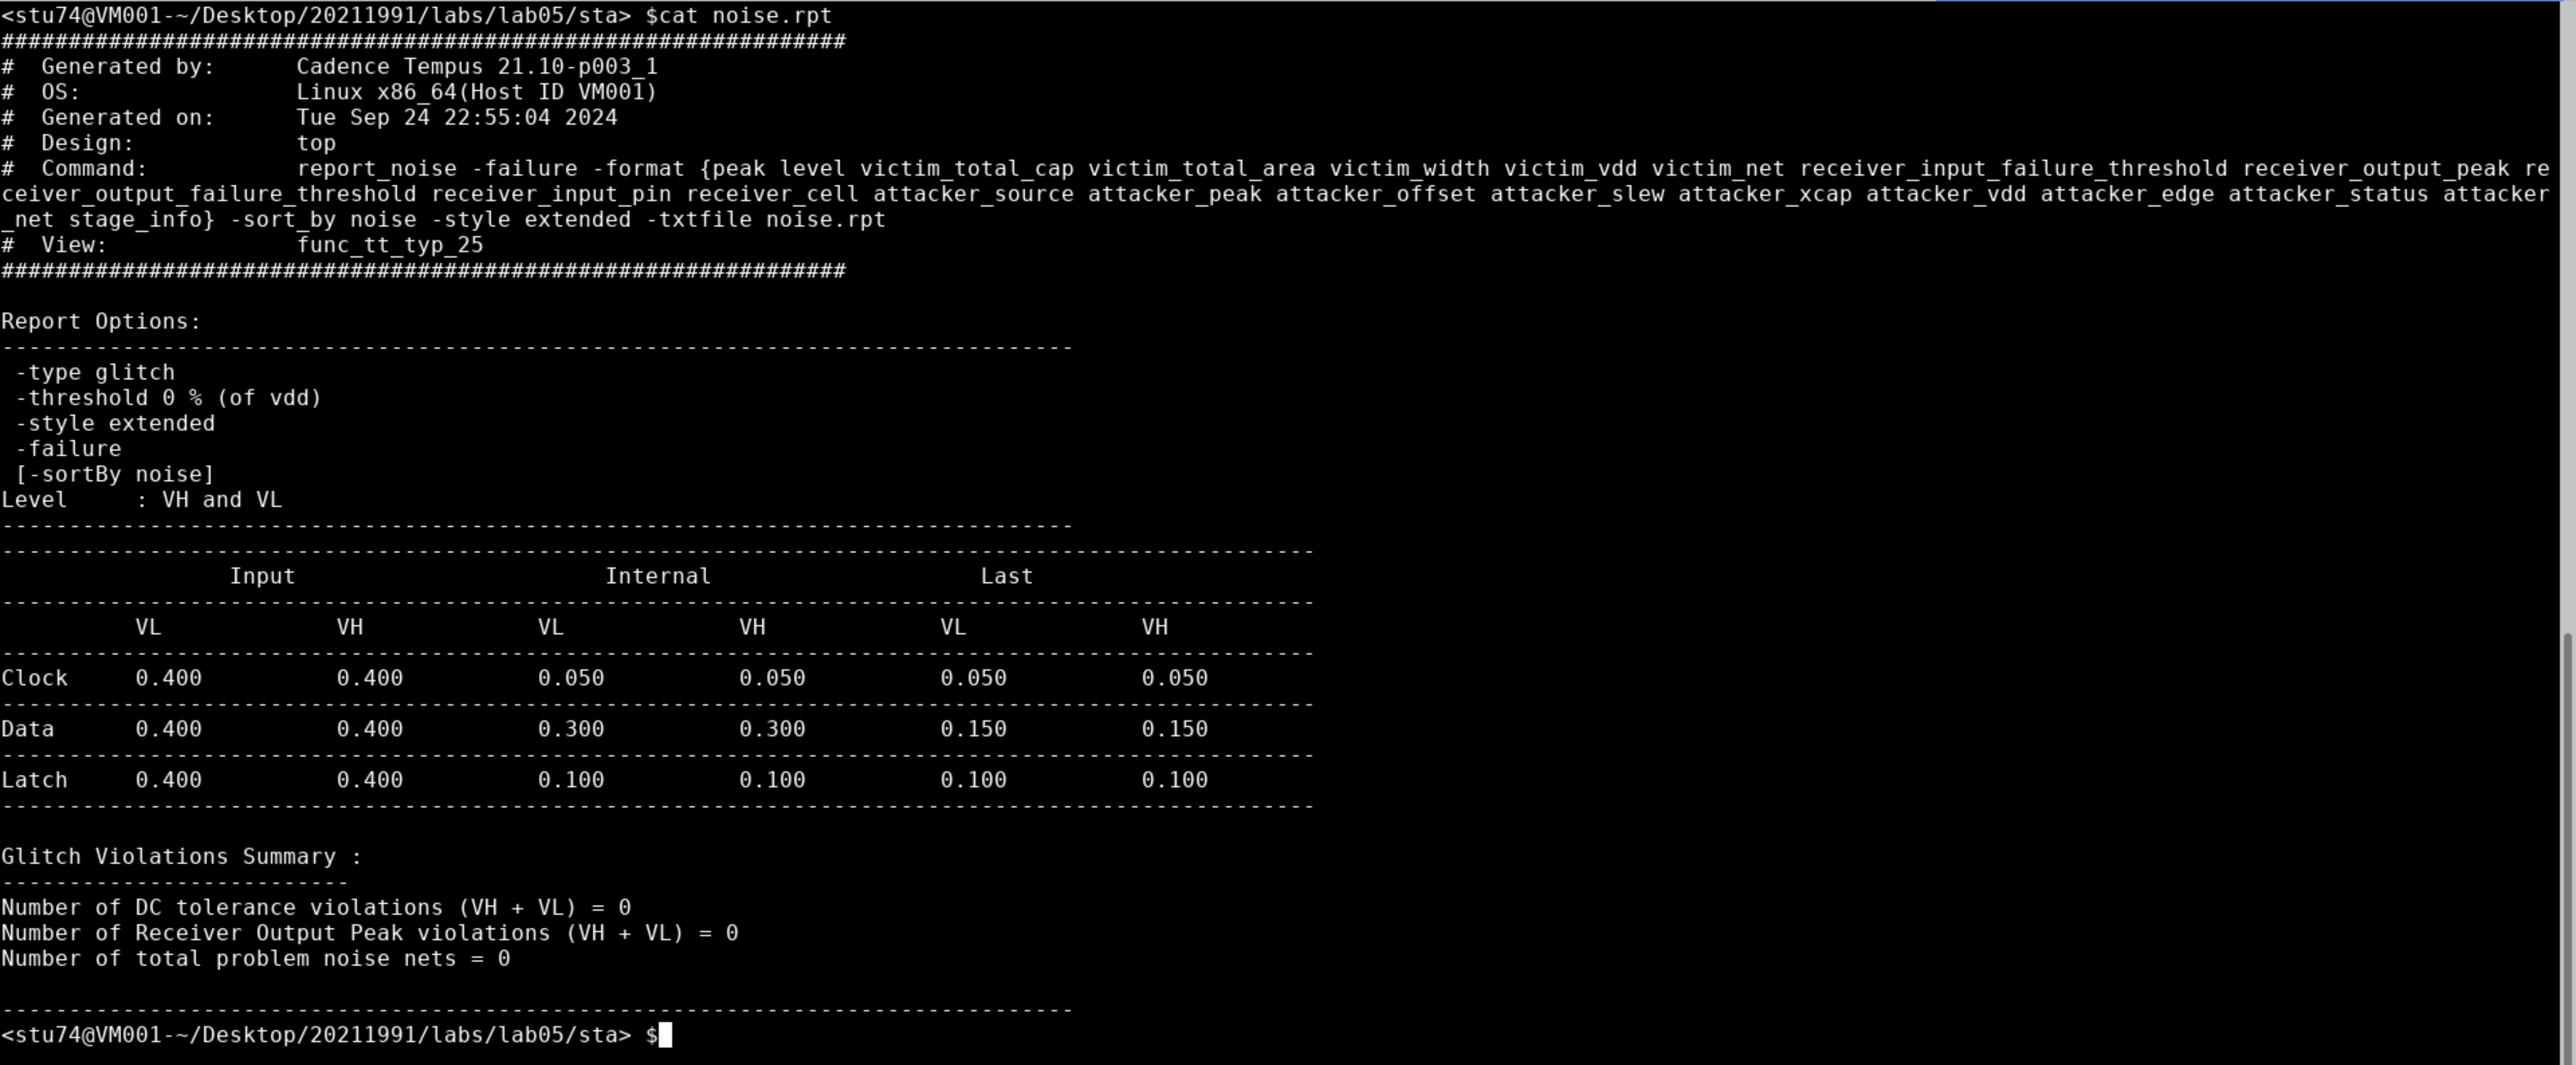
\includegraphics[width=0.8\textwidth]{images/lab05-06.png}
    \caption{lab05 图6}
\end{figure}

(无违例)

h)产生pulse width违例报告

\begin{figure}[H]
    \centering
    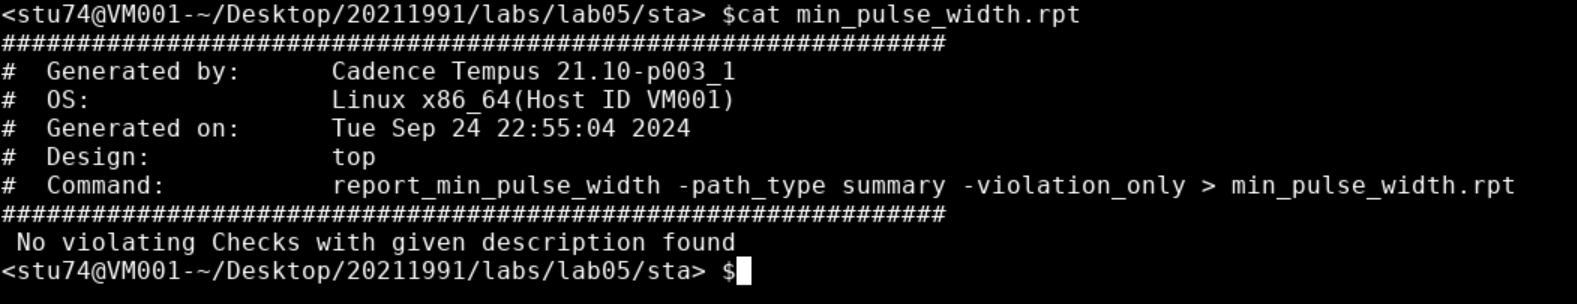
\includegraphics[width=0.8\textwidth]{images/lab05-07.png}
    \caption{lab05 图7}
\end{figure}

(无违例)

6、	保存Tempus时序database
 
7、	产生sdf文件,sdf包含了cell和net的真实延迟数据

\subsection{lab06}

实验目的

1、熟悉数字后端设计的流程。

2、熟悉使用TCL脚本使用innovus工具进行布局布线。

实验步骤:

1、	创建 mmmc 文件

创建 mmmc 文件,命名为 viewDefinition.tcl,各部分内容如下:

创建 library set
 
创建 rc corner
 
创建 delay corner
 
创建 constraint mode
 
创建 analysis view
 
2. 在 work 目录下启动 innovus,将设计导入进去

1)启动innovus

2)使用命令模式将设计导入

3)使用图形界面将设计导入

File→Import Design ,开始文件导入。Netlist→Verilog→alu.v
 
Technology/Physical Library→LEF Files,选择正确路径双击导入 lef 文件。需要注意tf目录下的 lef 文件需要第一个导入,macro目录下的 lef 文件需要第二个导入
 
Power→Power Nets 输入VDD ,Ground Nets 输入VSS 。VDD 是器件内部的工作电压,VSS 是电路公共接地端。
 
Analysis Configuration→viewDefinition.tcl 文件 
点击 OK ,导入设计

\begin{figure}[H]
    \centering
    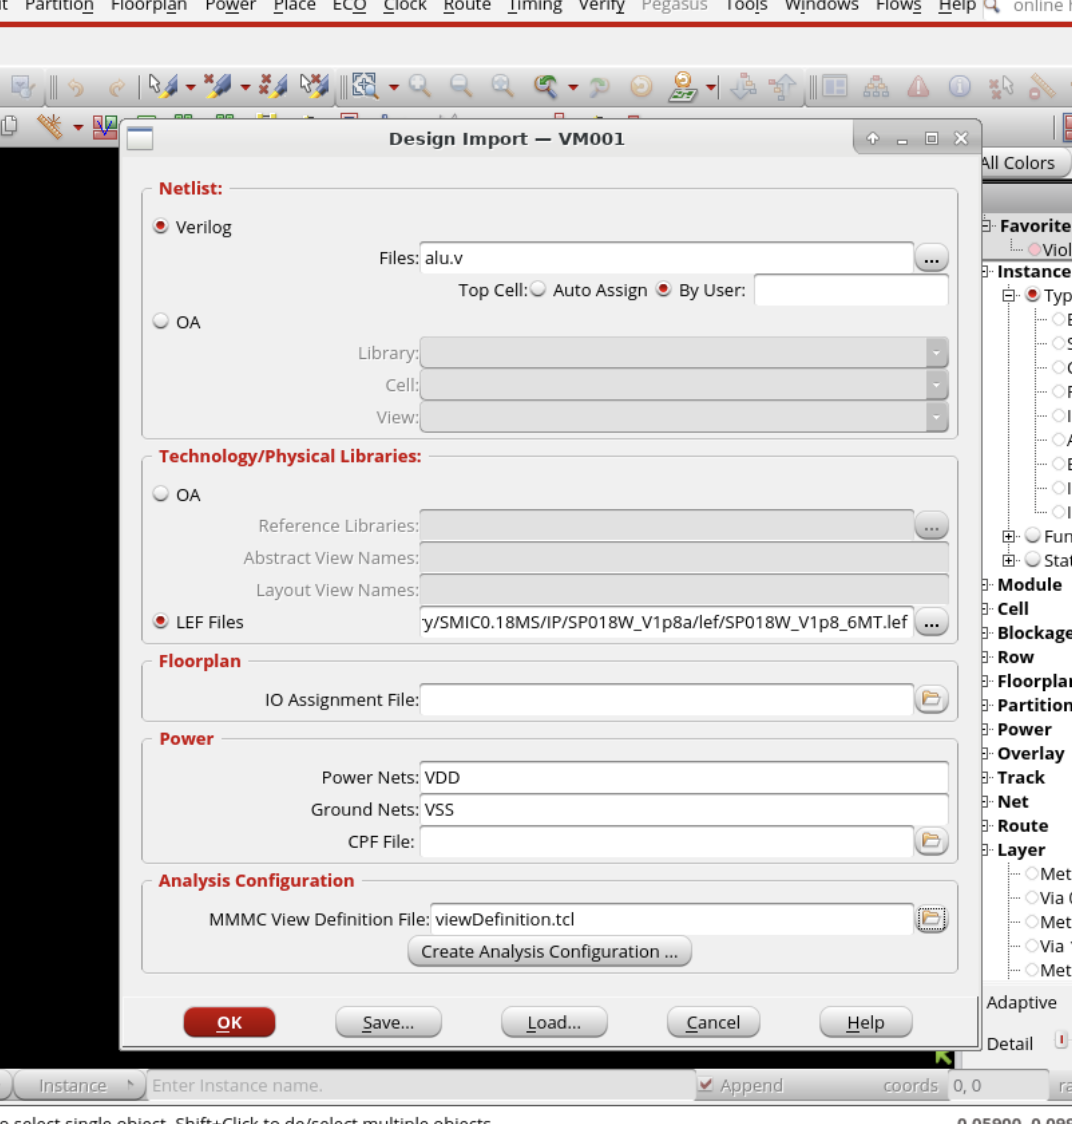
\includegraphics[width=0.8\textwidth]{images/lab06-01.png}
    \caption{lab06 图1}
\end{figure}
 
4)检查导入设计的错误

(a) 检查 innovus log 里面有没有 ERROR,特别是 load sdc 这一段

(b) 运行 \texttt{check\_timing -verbose > check.rpt},然后打开 check.rpt,只允许出现如下两种warning
 
(c) 运行 \texttt{timeDesign -prePlace},  报出 timing 情况
 
3.  完成布局规划

1) 制定芯片面积

命令模式
 
图形界面模式

Floorplan →Specify Floorplan  在 Basic 中选择Die/IO/Core Coordinates,三组坐标都设置为:0 0 205 210。点击OK
 
2) 完成 IO pin 分配

(a)添加 pin group
 
(b) 添加 Pin Guide

(c)摆放 IO Pins

3) 摆放 physical cell

(a)Endcap

(b)Welltap
 
4.  完成电源规划

1) 定义全局电源规划

Power→Global Net Connections
选中 Pin,分别连接 VDD 、VSS。
选中 Tie High,连接 VDD;
选中 Tie Low,连接 VSS。
每一次连接分别 Add to List,全部连接后 Apply,check ,无报错则全局电源连接成功
 
2) 添加 Power Stripe
    
3) 添加电源 follow pin

命令模式

图形界面模式
Route→Special Route
Net(s): VDD VSS
SRoute: Follow Pins

\begin{figure}[H]
    \centering
    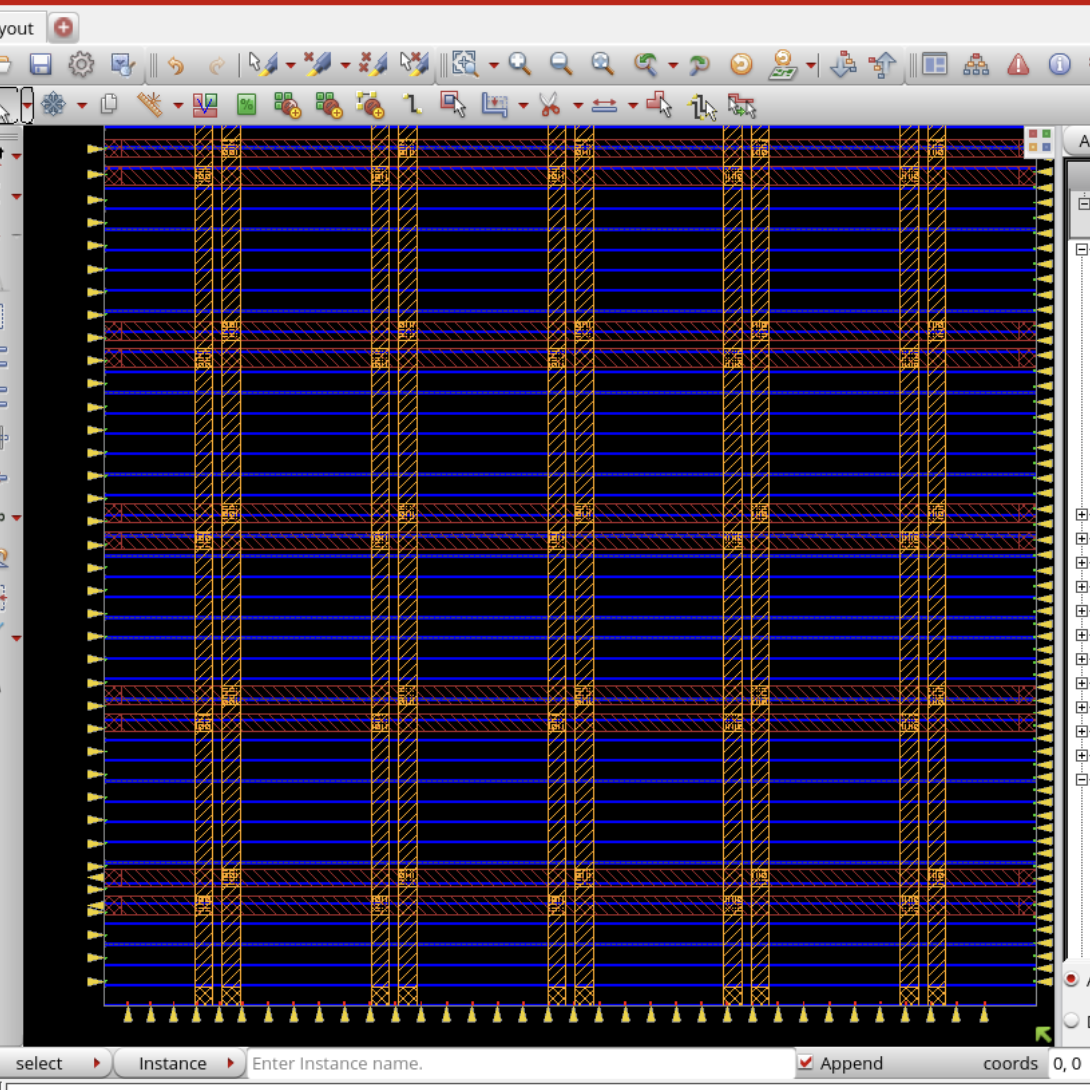
\includegraphics[width=0.8\textwidth]{images/lab06-03.png}
    \caption{lab06 图3}
\end{figure}

5. 保存数据

命令模式

saveDesign floorplan.enc

6. 完成plaecement

命令模式 \texttt{place\_opt\_design}

7. 检查place结果

Timing结果符合要求

8. CTS

1)\texttt{set\_ccoptc-property}

2)生成spec
  
3)运行cts
 
9. 检查CTS结果

Timing结果符合要求

10. Route

Route之前添加filler

\begin{figure}[H]
    \centering
    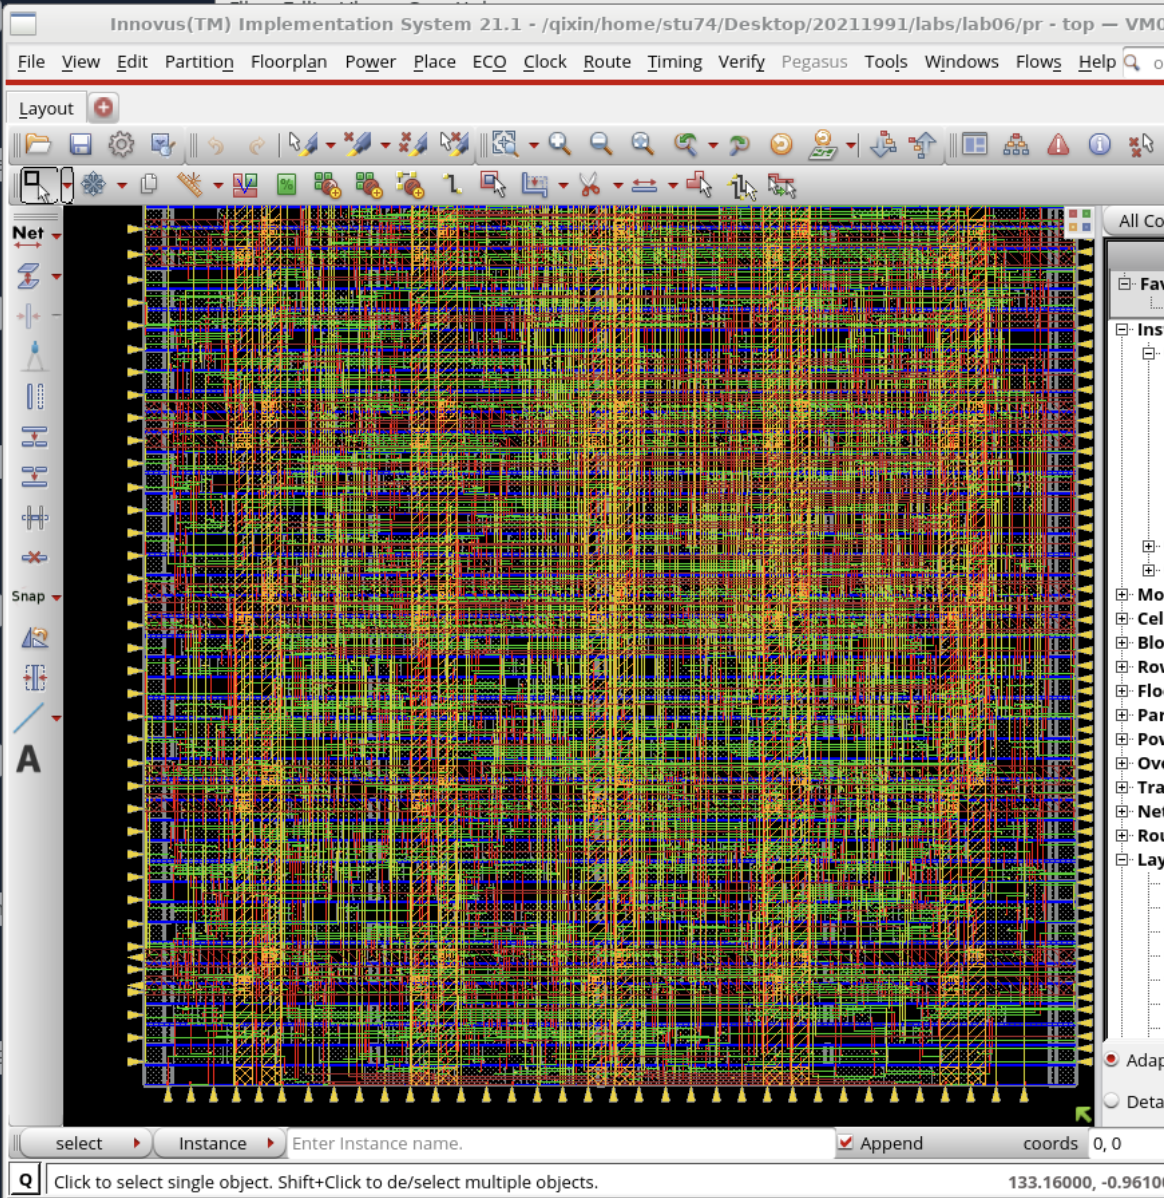
\includegraphics[width=0.8\textwidth]{images/lab06-04.png}
    \caption{lab06 图4}
\end{figure}

保存网表,命令:\texttt{saveNetlist route.v}
保存数据,命令:\texttt{saveDesign route.enc}
保存DEF,命令:\texttt{defOut -routing -withShield route.def}

\subsection{lab07}

实验步骤:

1. 将 def 文件导出,保存在 QRC 目录下;如 1 所示:

2. 打开 qrc.cmd 文件;如 2 所示:

3. 修改 qrc.cmd 文件中的内容:红色框中的部分,改成工艺库中 lef 文件所在的路径和第 一步保存的 def 文件的路径

4. 修改图中 1、2、3、4 处的内容:1 为需要提取的 corner;2 为提取的温度;3 为运行 提取出来的数据保存路径;4 为设计的名。修改完成后保存退出。

5. 进入到 \texttt{qrc\_tech\_dir} 目录下:

6. 打开 \texttt{qrc\_tech\_dir} 目录下的 corner.defs 文件,填写上需要抽取的 corner 的名字,与 第 4 部中的对应,后面填写 corner 文件的目录,填写正确后保存退出。

7. 使用 \texttt{qrc -cmd qrc.cmd},运行 qrc,如图所示:

8. QRC 提取运行完成:

\begin{figure}[H]
    \centering
    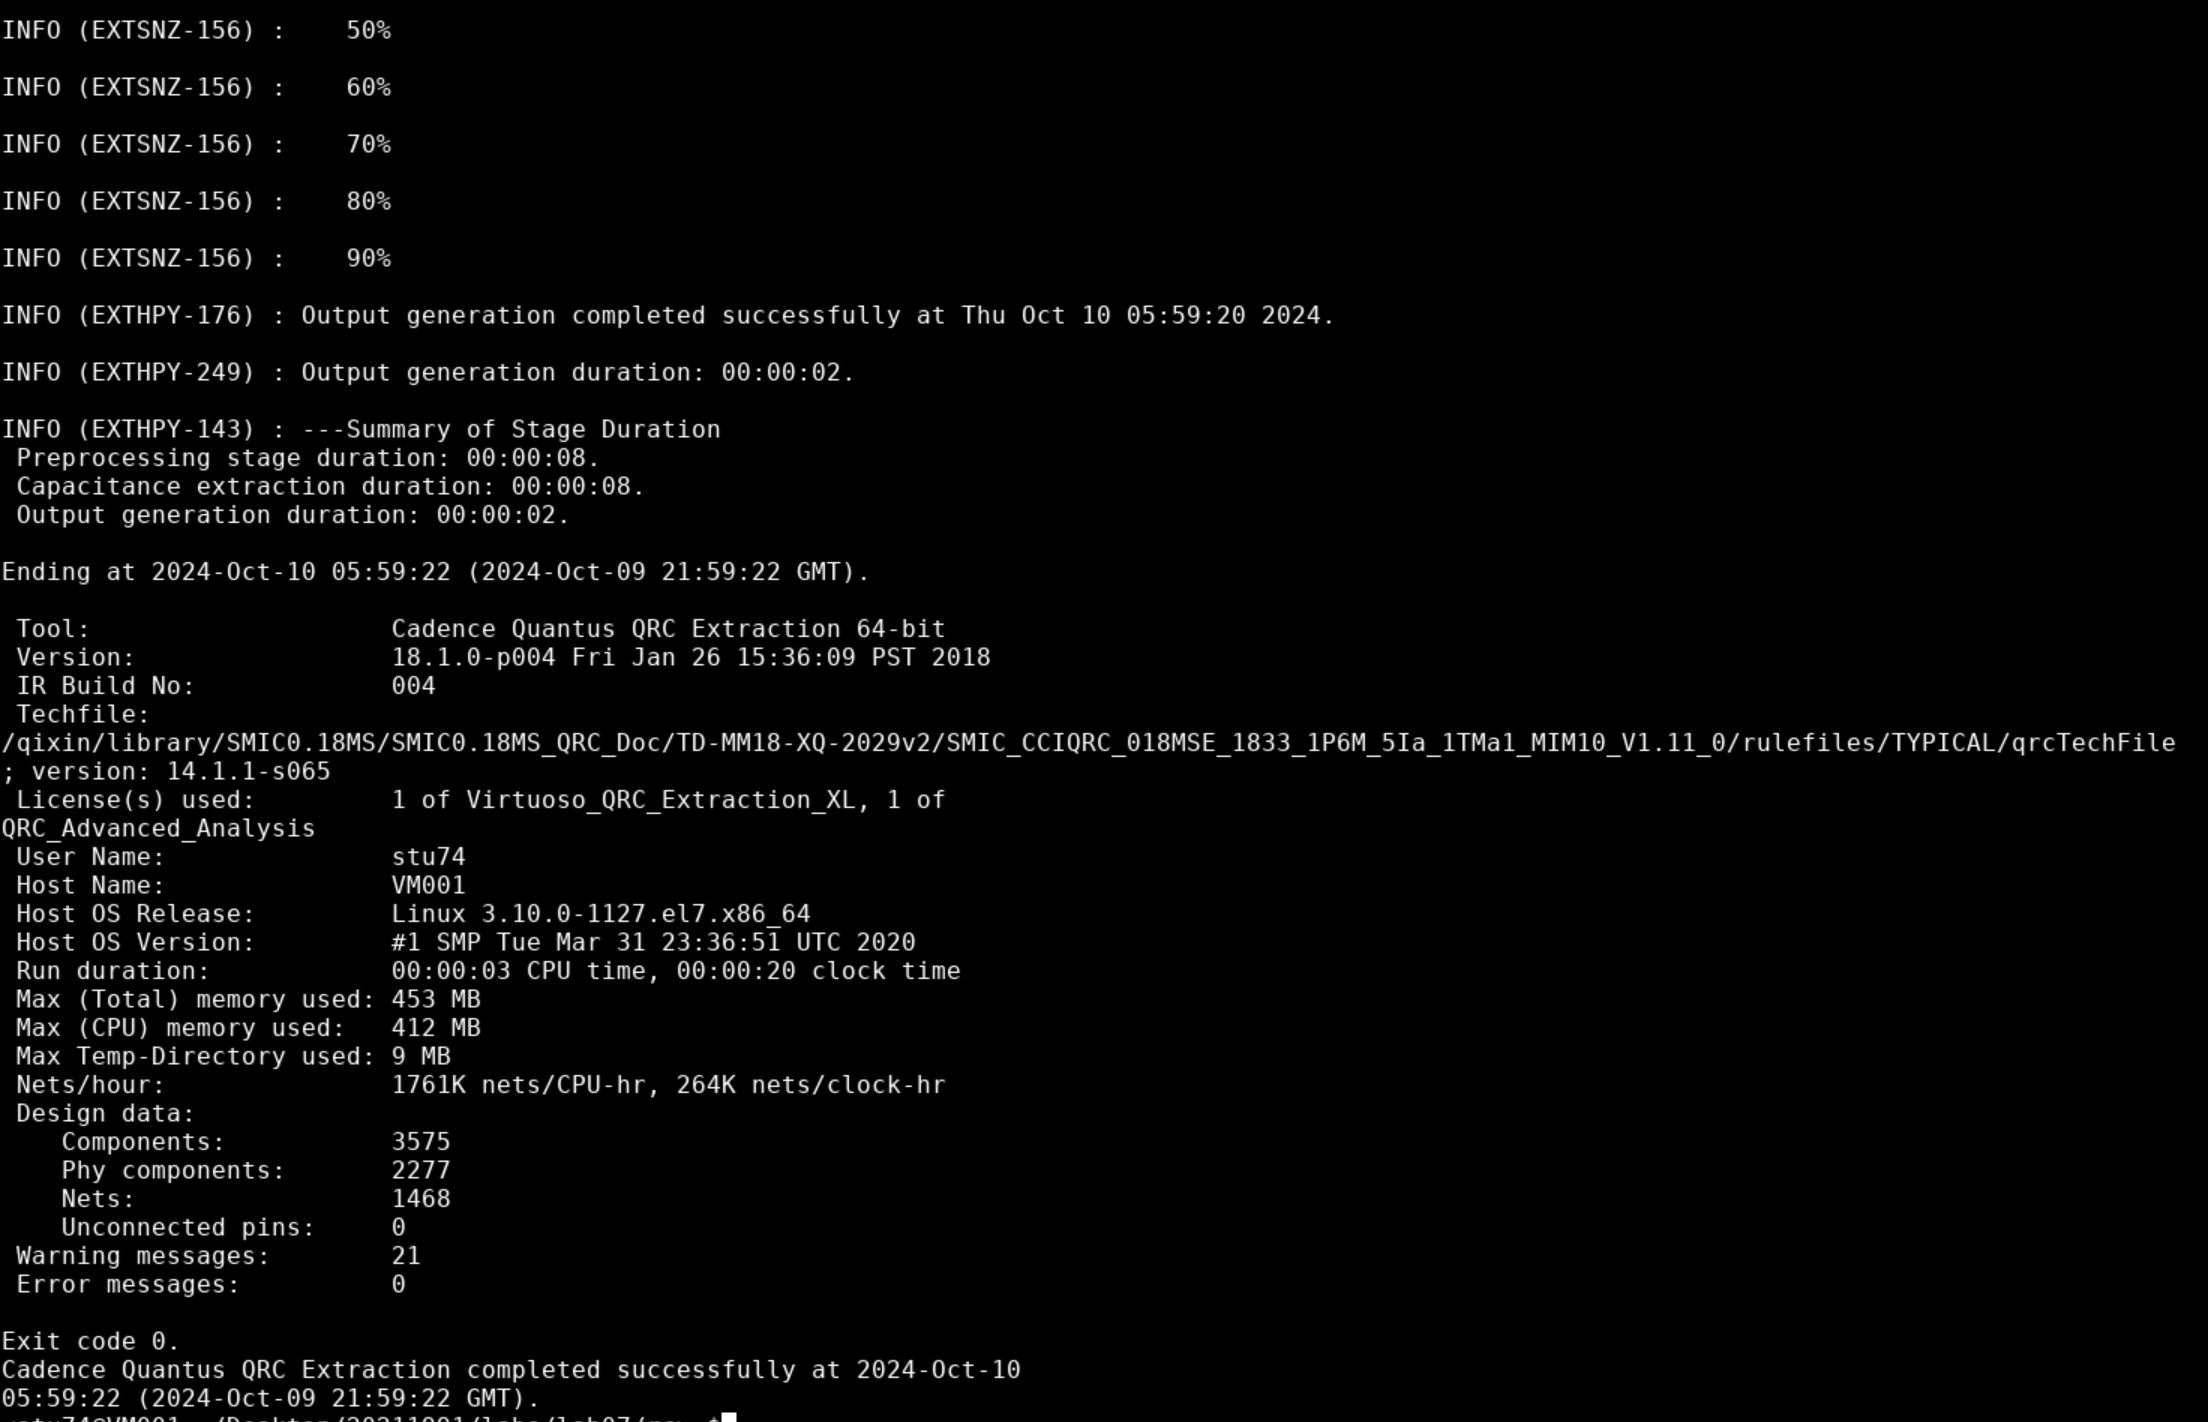
\includegraphics[width=0.8\textwidth]{images/lab07-01.png}
    \caption{lab07 图1}
\end{figure}

9. 进入到 \texttt{qrc\_test} 目录中,里面为提取出的寄生参数文件:ALU.spef

\subsection{lab08}

实验目的

1、掌握 pr 工具修复 metal 的 drc

2、掌握 drc flow 和 lvs flow

实验步骤

DRC 部分

1. innovus 工具修 innovus 中导入 route 后的数据(即 pr 部分保存的 route.enc),键入:工具会全局修复 70\%-80\%的违例

2. add Metal Fill

3. StreamOut(innovus) 导出 GDS 文件,内容如下:

其中.gz 文件会进行自动压缩;如果没有指定-mapfile 会自动生成一个 streamOut.map 的 模板文件,需要修改;streamOut.map 是 layer name 和 layer number 的对应关系,可以 在 DRM(design rule manual)中找到(此处文件已修改) 对应关系也可以来自于 Calibre drc rule deck:

steamOut.map 手改后的部分内容如下:

4. Merge GDS(Calibre) 将金属层 GDS 和标准单元 GDS 合并起来

a)在 drc 路径下新建一个 merge.tcl 脚本,内容如下:

b)运行脚本,会生成合并后的 gds:

c)查看 merge 后的 gds:

(此处无 cell not defined,empty cell used 的 warning 表示 merge 成功了)

\begin{figure}[H]
    \centering
    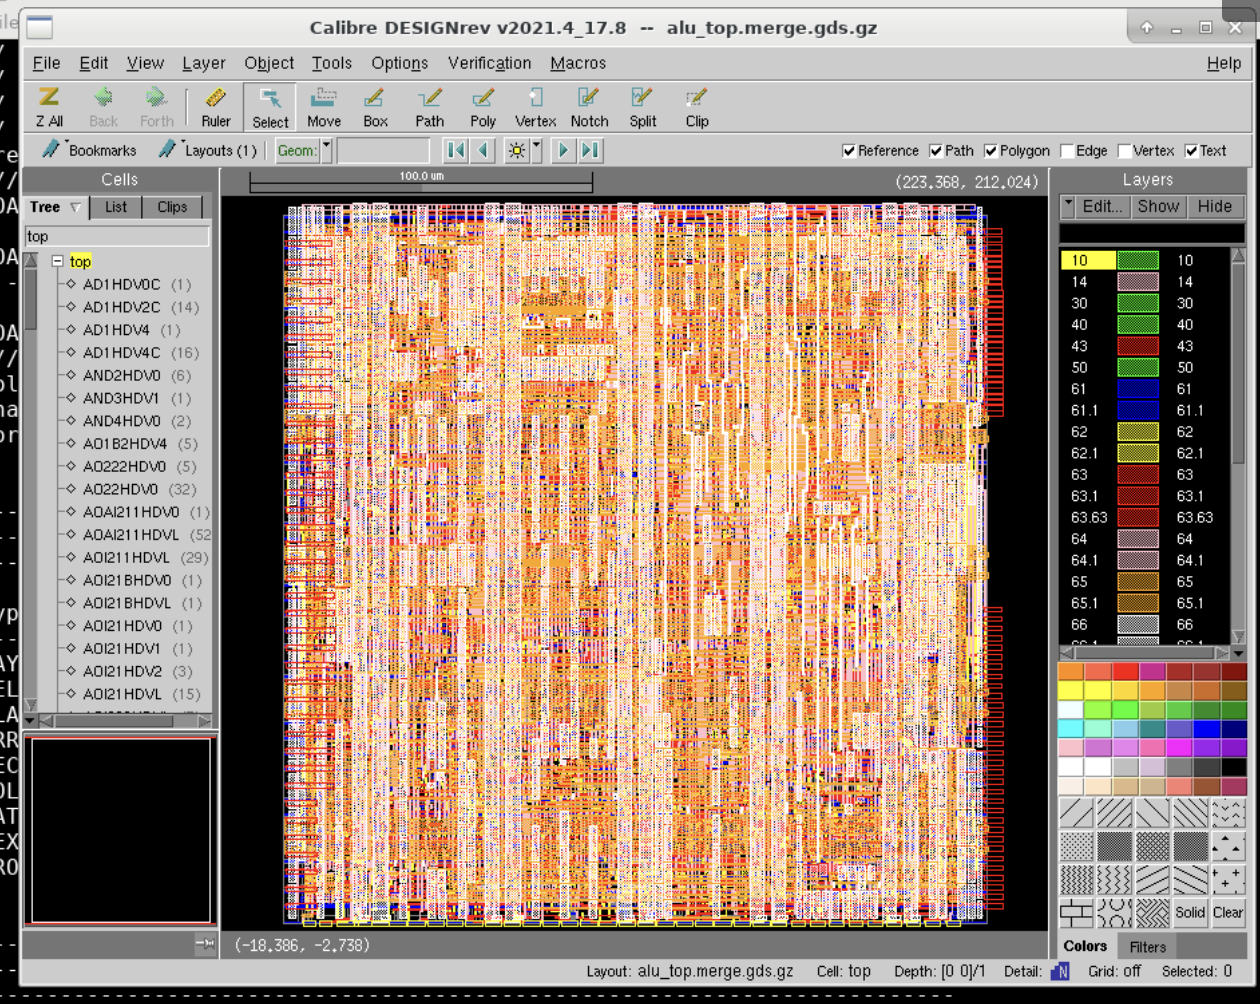
\includegraphics[width=0.8\textwidth]{images/lab08-01.png}
    \caption{lab08 图1}
\end{figure}

此时这边命名是乱的,打开 GDS 后右侧 layer name 默认显示的是 layer number,可以通 过三种方式导入对应的 drc rule check: (1)通过“load input SVRF Layer Names”导入对应的 drc rule check(推荐)

(2) 通过“save layer properties”保存 layer number 和 layer name 的对应关系到一个 文件中,下次可以“load layer properties”,layer properties load 速度比 SVRF load 速度快。此时目录保存会生成一个 properties 文件,gvim 文件可得到他们的对应关 系,下次打开更加方便。

gvim 文件可得到他们的对应关系:

(对应关系)

calibredrv 打开界面后,load properties,生成正确的对应关系且速度更快:

(3)也可以点击“save as default”,工具会把 layer properties 存到下面隐藏目录,下次打 开 calibredrv 会自动加载 layerprops:

保存文件及路径:

5. set rule deck(calibre) 打开 drc 文件,修改参数: 转换到底层命令模式,键入“?LAYOUT”,查找修改对象:

修改后:

6. run DRC(calibre)

7. calibre debug

a)用 RVE 查看 DRC 结果的方法: 用 calibredrv 打开 GDS 后,点击 Verification→Srart RVE

b)innovus 中查看 drc 结果的方法: 打开 violation browser 按钮 ,点击 loadreport:

文件类型选择 calibre,文件名选择之前保存的 database:

LVS 部分:

1.merge netlist

2. merge gds 即 DRC 部分 calibre merge gds 以后的 gds 文件,将其复制到当前目录

3. hcell list Innovus 里运行以下命令,得到 hcell mapping list

5. run lvs

report 保存在 lvs.rep 文件中

6. calibre lvs debug Calibre 里 lvs 所有信息存放在 svdb 数据库中 查看 debug lvs 结果:

\begin{figure}[H]
    \centering
    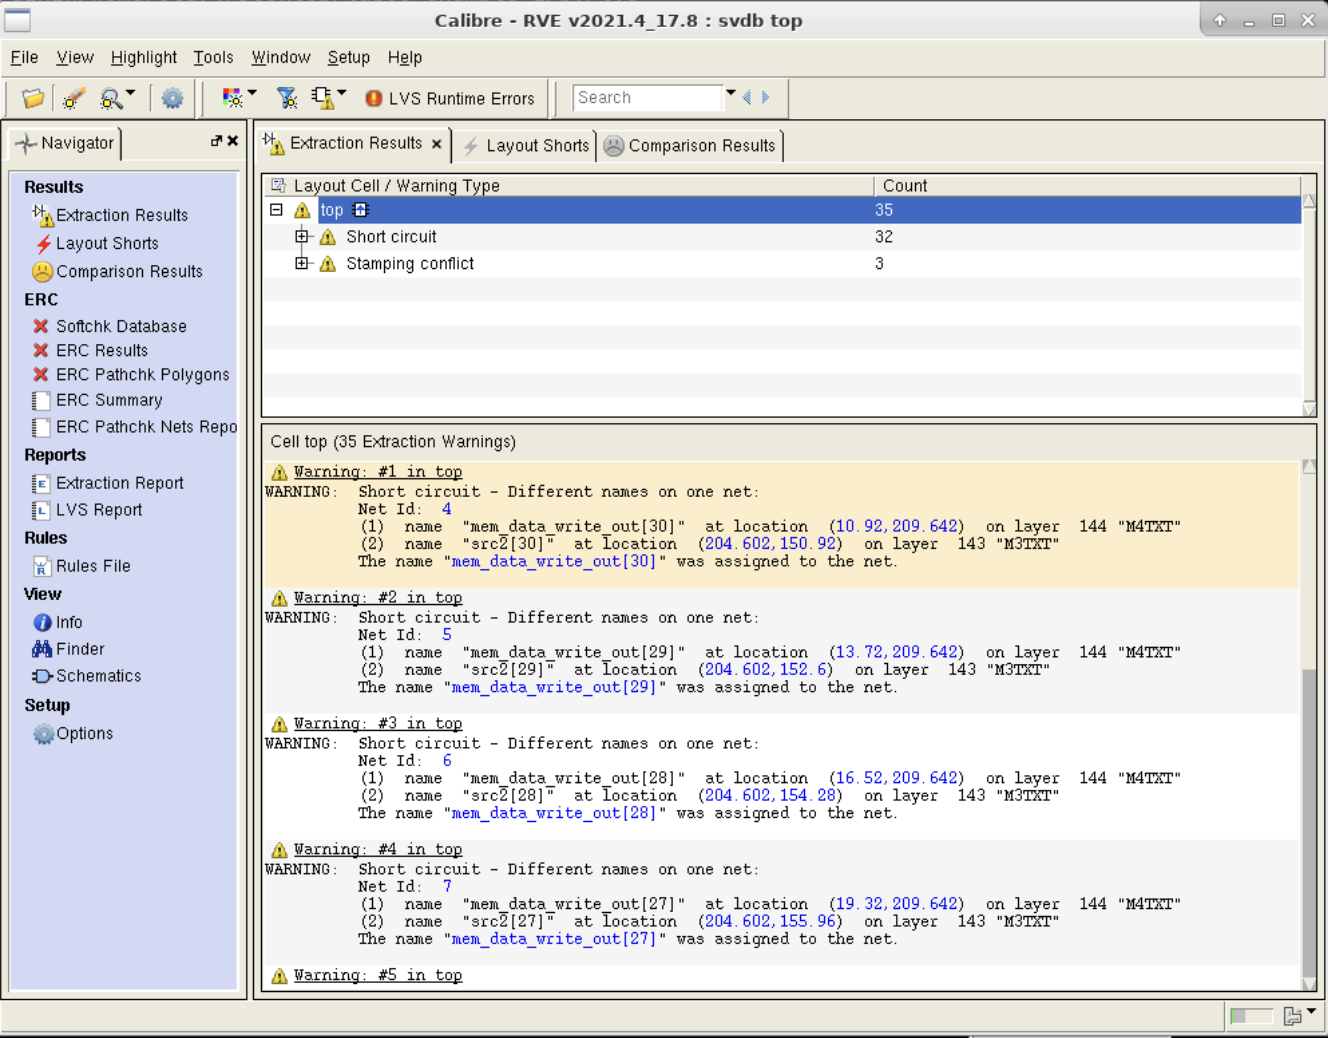
\includegraphics[width=0.8\textwidth]{images/lab08-02.png}
    \caption{lab08 图2}
\end{figure}

\section{总结}

本课程通过多个实验模块系统介绍了IC设计流程,涵盖Verilog语言应用、ALU设计与测试、仿真工具使用、逻辑综合、形式验证及优化等环节。学习了如何编写模块化设计与Testbench进行功能验证,并使用Design Compiler通过TCL脚本完成综合和时序分析,掌握了寄生参数的提取及逻辑优化方法。实验培养了实践能力和对IC设计工具的熟练应用,为未来在集成电路设计领域的研究和工作奠定了坚实基础。
